% !TEX TS-program = pdflatex
% !TEX encoding = UTF-8 Unicode

\documentclass[11pt]{report} % use larger type; default would be 10pt

\usepackage[utf8]{inputenc} % set input encoding (not needed with XeLaTeX)
\usepackage[czech]{babel}

%%% PAGE DIMENSIONS
\usepackage{geometry} % to change the page dimensions
\geometry{a4paper} % or letterpaper (US) or a5paper or....
\geometry{top=45 px, left=65px,right=65px,bottom=55px} % for example, change the margins to 2 inches all round

\usepackage{graphicx} % support the \includegraphics command and options
\usepackage{hyperref}
\usepackage{indentfirst}
\usepackage{float}
\usepackage{listings}
\usepackage{xfrac}
\usepackage{amsmath, amsthm, amssymb}
\usepackage{mathtools}
\usepackage{array}

\newcommand{\R}{\mathbb{R}}
\newcommand{\N}{\mathbb{N}}
\renewcommand{\vec}[1]{\mathbf{#1}}

\newtheorem{theorem}{Věta}[section]

\newtheorem{implication}{Důsledek}[section]

\makeatletter
\newcommand{\dotminus}{\mathbin{\text{\@dotminus}}}

\newcommand{\@dotminus}{%
	\ooalign{\hidewidth\raise1ex\hbox{.}\hidewidth\cr$\m@th-$\cr}%
}
\makeatother

\lstset
{ %Formatting for code in appendix
	numbers=left,
	stepnumber=1,
	tabsize = 4
}
\usepackage{wrapfig}

%%% The "real" document content comes below...


\begin{document}
	
\tableofcontents
\part{Společné povinné okruhy}
\chapter{Základy složitosti a vyčíslitelnosti}
\section{Výpočetní modely (Turingovy stroje, RAM).}
\subsection{Turingův stroj}
\textbf{(Jednopáskový deterministický) Turingův stroj (TS)} $M$ je pětice
$$M = (Q, \Sigma, \delta, q_0, F)$$
\begin{itemize}
	\leftskip 40pt
	\setlength{\itemsep}{0pt}
	\item $Q$ je konečná \textbf{množina stavů}.
	\item $\Sigma$ je konečná \textbf{pásková abeceda}, která obsahuje znak $\lambda$ pro prázdné políčko. (Často budeme rozlišovat \textbf{páskovou (vnitřní)} a \textbf{vstupní (vnější) abecedu}.)
	\item $\delta : Q \times \Sigma \mapsto Q \times \Sigma \times \{R, N, L\} \cup {\bot}$ je \textbf{přechodová funkce},
	kde $\bot$ označuje nedefinovaný přechod.
	\item $q_0 \in Q$ je \textbf{počáteční stav}.
	\item $F \subseteq Q$ je \textbf{množina přijímajících stavů}.
\end{itemize}

Turingův stroj sestává z \textbf{řídící jednotky}, \textbf{pásky}, která je potenciálně nekonečná v obou směrech, a
\textbf{hlavy} pro čtení a zápis, která se pohybuje oběma směry.

\textbf{Displej} je dvojice $(q, a)$, kde $q \in Q$ je aktuální stav Turingova stroje a $a \in \Sigma$ je symbol pod hlavou. Na základě displeje TS rozhoduje, jaký další krok má vykonat.

\textbf{Konfigurace} zachycuje stav výpočtu Turingova stroje a skládá se ze
\begin{itemize}
	\leftskip 40pt
	\setlength{\itemsep}{0pt}
	\item stavu řídící jednotky
	\item slova na pásce (od nejlevějšího do nejpravějšího neprázdného políčka)
	\item pozice hlavy na pásce (v rámci slova na této pásce)
\end{itemize}

\subsubsection{Výpočet TS}
\textbf{Výpočet} zahajuje TS $M$ v \textbf{počáteční konfiguraci}, tedy v počátečním stavu se vstupním slovem zapsaným na pásce a hlavou nad nejlevějším symbolem vstupního slova. Vstupní slovo nesmí obsahovat prázdné políčko. Pokud se $M$ nachází ve stavu $q \in Q$ a pod hlavou je symbol $a \in \Sigma$, pak krok výpočtu probíhá následovně:
\begin{enumerate}
	\leftskip 40pt
	\setlength{\itemsep}{0pt}
	\item Je-li $\delta(q, a) = \bot$, výpočet $M$ končí,
	\item Je-li $\delta(q, a) = (q', a', Z)$, kde $q' \in Q$, $a' \in \Sigma$ a $Z \in \{L, N, R\}$, přejde $M$ do stavu $q'$, zapíše na pozici hlavy symbol $a'$ a pohne hlavou doleva (pokud $Z = L$), doprava (pokud $Z = R$), nebo hlava zůstane stát (pokud $Z = N$).	
\end{enumerate}

TS $M$ \textbf{přijímá slovo} $w$, pokud výpočet $M$ se vstupem $w$ skončí a $M$ se po ukončení výpočtu nachází v přijímajícím stavu. 

TS $M$ \textbf{odmítá slovo} $w$, pokud výpočet $M$ nad vstupem $w$ skončí a $M$ se po ukončení výpočtu nenachází v přijímajícím stavu. 

Fakt, že výpočet $M$ nad vstupním slovem $w$ skončí, označíme pomocí $M(w){\downarrow}$ a řekneme, že výpočet \textbf{konverguje}. 

Fakt, že výpočet $M$ nad vstupním slovem $w$ nikdy neskončí, označíme pomocí $M(w){\uparrow}$ a řekneme, že výpočet \textbf{diverguje}.

\subsubsection{Turingovsky rozhodnutelné jazyky}
\textbf{Jazyk slov přijímaných} TS $M$ označíme pomocí $L(M)$. 

Řekneme, že jazyk $L$ je \textbf{částečně (Turingovsky) rozhodnutelný} (též \textbf{rekurzivně spočetný}), pokud existuje
Turingův stroj $M$, pro který $L = L(M)$.

Řekneme, že jazyk $L$ je \textbf{(Turingovsky) rozhodnutelný} (též \textbf{rekurzivní}), pokud existuje Turingův stroj $M$, který se \textit{vždy zastaví} a $L = L(M)$.

\subsubsection{Turingovsky vyčíslitelné funkce}
Turingův stroj $M$ s páskovou abecedou $\Sigma$ \textbf{počítá} nějakou \textit{částečnou} funkci $f_M : \Sigma^* \mapsto \Sigma^*$ (částečná = pro některé vstupy není definovaná). Pokud $M(w){\downarrow}$ pro daný vstup $w \in \Sigma^*$, je hodnota funkce $f_M(w)$ \textbf{definovaná}, což označíme pomocí $f_M(w){\downarrow}$. \textbf{Hodnotou funkce} $f_M(w)$ je potom slovo na (výstupní) pásce $M$ po ukončení výpočtu nad $w$. Pokud $M(w){\uparrow}$, pak je hodnota $f_M(w)$ \textbf{nedefinovaná}, což označíme pomocí $f_M(w){\uparrow}$. 

Funkce $f : \Sigma^* \mapsto \Sigma^*$ je \textbf{turingovsky vyčíslitelná}, pokud existuje Turingův stroj \textbf{M}, který ji počítá. \textbf{\textit{Každá turingovsky vyčíslitelná funkce má nekonečně mnoho různých Turingových strojů, 	které ji počítají!}}

\subsubsection{Varianty TS}
Turingovy stroje mají řadu variant, například:
\begin{itemize}
	\leftskip 40pt
	\setlength{\itemsep}{0pt}
	\item TS s jednosměrně nekonečnou páskou
	\item TS s více páskami (vstupní/výstupní/pracovní)
	\item TS s více hlavami na páskách
	\item TS s pouze binární abecedou
	\item nedeterministické TS
\end{itemize}
Zmíněné varianty jsou ekvivalentní \uv{našemu} modelu v tom smyslu, že všechny přijímají touž třídu jazyků a vyčíslují touž třídu funkcí.

\textbf{$k$-páskový Turingův stroj} se od jednopáskového Turingova stroje líší následujícím způsobem:
\begin{itemize}
	\leftskip 40pt
	\setlength{\itemsep}{0pt}
	\item Má $k$ pásek, na každé je zvláštní hlava.
	\begin{itemize}
		\leftskip 40pt
		\setlength{\itemsep}{0pt}	
		\item Vstupní páska na počátku obsahuje vstupní řetězec. Často je určena jen pro čtení.
		\item Pracovní pásky jsou určeny pro čtení i zápis.
		\item Výstupní páska na konci obsahuje výstupní řetězec. Často je určena jen pro zápis s pohybem hlavy jen vpravo.
	\end{itemize}
	\item Hlavy na páskách se pohybují nezávisle na sobě.
	\item Přechodová funkce je typu
		$$\delta : Q \times \Sigma^k \mapsto Q \times \Sigma^k \times \{R, N, L\}^k \cup {\bot}$$
\end{itemize}

Neplést \textit{multi-tape (vícepáskové)} a \textit{multi-track} TS. Druhé jmenované mají také více pásek, ale \textit{jedinou hlavu společnou pro všechny}.

\begin{theorem}
Ke každému $k$-páskovému Turingovu stroji $M$ existuje jednopáskový Turingův stroj $M'$, který simuluje práci $M$, přijímá týž jazyk jako $M$ a počítá touž funkci jako $M$.
\end{theorem}
\begin{proof}
	Pouze idea. Chceme simulovat $k$-páskový na jednopáskovém. Dvě varianty:
	\begin{enumerate}
		\leftskip 40pt
		\setlength{\itemsep}{0pt}
		\item Obsahy pásek zapíšeme na jedinou, oddělíme je novým symbolem $\#$. Pozice hlav označuje speciální značka, např. je-li hlava nad symbolem $0$, označíme to pomocí $\overline{0}$ -- v praxi to znamená pro každý symbol přidat do abecedy jeho označkovanou variantu, tj. $|\Sigma|$ nových symbolů. Dojde-li nějaké pásce místo, musí se všechny symboly vpravo od ní posunout.
		
		\item Vytvoříme novou abecedu $\Sigma'$ jako kartézský součin $k$ abeced, tj. $\Sigma' = \Sigma^k$. Jeden symbol tedy reprezentuje $k$-tici původních symbolů. Je taky potřeba ošetřit pozici hlav.
	\end{enumerate}
\end{proof}

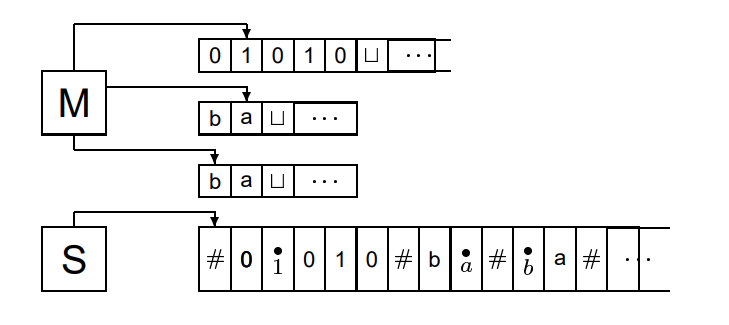
\includegraphics[width=0.6\textwidth]{img/turing_multi_seq.png}

\subsection{RAM (Random Access Machine)}
\begin{wrapfigure}{r}{0.4\textwidth}
	\centering
	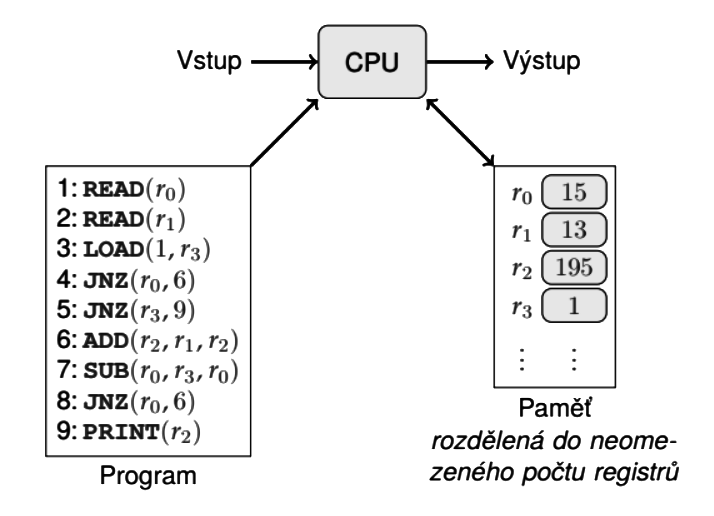
\includegraphics[width=0.35\textwidth]{img/ram.png}
\end{wrapfigure}
RAM je stroj s náhodným přístupem do paměti. Jde o model, který se často používá jako základní výpočetní model při měření časové i prostorové složitosti algoritmů. Cílem bylo vytvořit model, který by se co nejvíce blížil reálným počítačům. Podobně jako Turingovy stroje, i RAM je strojem s \textbf{oddělenou pamětí pro data a pro instrukce}, nejedná se tedy o stroje Von Neumannovy architektury. 

\textbf{Program} pro RAM je konečnou posloupností instrukcí $P = I_0, I_1, I_2, \dots I_l$

Paměť pro data se skládá z neomezené posloupnosti registrů $r_i, i \in \mathbb{N}$ Obsahem registru může být libovolně velké přirozené číslo. Při popisu instrukcí budeme dodržovat následující konvence:
\begin{itemize}
	\leftskip 20pt
	\setlength{\itemsep}{0pt}
	\item Obsah registru $r_i$ budeme označovat pomocí $[r_i]$.
	\item Nepřímá adresace (tj. obsahem jiného registru) pomocí $[[r_i]] = [r_{[r_j]}]$. 
	\item Přiřazení hodnoty $c$ do registru $r_i$ označíme $r_i \leftarrow c$
\end{itemize}

Seznam instrukcí pro RAM viz tabulka \ref{ram_instrukce}.
\begin{table}[H]
	\centering
	\renewcommand{\arraystretch}{1.5}
	\begin{tabular}{|l|l|}
		\hline
		LOAD($C, r_i$) 			& $r_i \leftarrow C$ 							\\ \hline
		ADD($r_i, r_j, r_k$) 	& $r_k \leftarrow [r_i] + [r_j]$				\\ \hline
		SUB($r_i, r_j, r_k$) 	& $r_k \leftarrow [r_i] \dotminus [r_j]$\quad ($x \dotminus y = max(x-y, 0)$)    	\\ \hline
		COPY($[r_p], r_d$) 		& $r_d \leftarrow [[rp]]$				 		\\ \hline
		COPY($r_s,[r_d]$) 		& $r_{[r_d]} \leftarrow [r_s]$                  \\ \hline
		JNZ($r_i, I_z$) 		& if $[r_i] > 0$ then goto instruction $I_z$ 	\\ \hline
		READ($r_i$) 			& $r_i \leftarrow$ input						\\ \hline
		PRINT($r_i$) 			& output $\leftarrow [r_i]$   					\\ \hline
	\end{tabular}
	\caption{Seznam instrukcí RAM}
	\label{ram_instrukce}
\end{table}

\subsubsection{Jazyky rozhodnutelné RAM}
Uvažme abecedu $\Sigma = \{\sigma_1, \sigma_2, \dots, \sigma_k\}$. Slovo $w = \sigma_{i_1}, \sigma_{i_2} \dots \sigma_{i_n}$ předáme RAMu $R$ jako posloupnost čísel $i_1, \dots, i_n$. Konec slova pozná $R$ díky tomu, že READ načte 0, není-li už k dispozici vstup.

RAM $R$ \textbf{přijme} slovo $w$, pokud $R(w){\downarrow}$ a první číslo, které $R$ zapíše na výstup je 1.

RAM $R$ \textbf{odmítne} slovo w, pokud $R(w){\downarrow}$ a $R$ buď na výstup nezapíše nic, nebo první zapsané číslo je jiné než 1.

\textbf{Jazyk slov přijímaných RAMem} $R$ označíme pomocí $L(R)$. 

Pokud pro jazyk $L$ platí, že $L = L(R)$ pro nějaký RAM, pak řekneme, že je \textbf{částečně rozhodnutelný (RAMem)}. Pokud se navíc výpočet $R$ \textit{nad každým vstupem zastaví}, řekneme, že je $L = L(R)$ \textbf{rozhodnutelný (RAMem)}.

\subsubsection{Funkce vyčíslitelné na RAMu}
O RAMu $R$ řekneme, že \textbf{počítá} částečnou \textit{aritmetickou} funkci $f : \N^n \mapsto \N, n \geq 0$, pokud za předpokladu, že $R$ dostane na vstup $n$-tici $(x_1, \dots, x_n)$, platí následující:
\begin{itemize}
	\leftskip 20pt
	\setlength{\itemsep}{0pt}
	\item Je-li $f(x_1, \dots, x_n){\downarrow}$, pak $R(x_1, \dots, x_n){\downarrow}$ a $R$ vypíše na výstup hodnotu $f(x_1, \dots, x_n)$.
	\item Je-li $f(x_1, \dots, x_n){\uparrow}$, pak $R(x_1, \dots, x_n){\uparrow}$.
\end{itemize}
O funkci $f$, pro niž existuje RAM, který ji počítá, řekneme, že je \textbf{vyčíslitelná na RAMu}.

\subsubsection{Řetězcové (string) funkce vyčíslitelné na RAMu}
RAM $R$ \textbf{počítá} částečnou (\textit{řetězcovou}) funkci $f : \Sigma^* \mapsto \Sigma^*$, kde $\Sigma = \{\sigma_1, \sigma_2, \dots, \sigma_k\}$, pokud platí:
\begin{itemize}
	\leftskip 20pt
	\setlength{\itemsep}{0pt}
	\item Vstupní řetězec $w = \sigma_{i_1}\sigma_{i_2}\dots\sigma_{i_n}$ je předaný jako posloupnost čísel $i_1, \dots, i_n$.
	\item Konec slova pozná $R$ díky tomu, že READ načte 0, není-li už k dispozici vstup.
	\item Pokud je $f(w){\downarrow}= \sigma_{j_1}\sigma_{j_2}\dots\sigma_{j_m}$, pak $R(w){\downarrow}$ a na výstup je
	zapsaná posloupnost čísel $j_1, j_2, \dots, j_m, 0$.
	\item Pokud $f(w){\uparrow}$, pak $R(w){\uparrow}$.
\end{itemize}
O funkci $f$, pro níž existuje RAM $R$, který ji počítá, říkáme, že je \textbf{vyčíslitelná na RAMu}.

\subsubsection{Programování na RAMu}
Programy pro RAM odpovídají procedurálnímu jazyku:
\begin{itemize}
	\leftskip 20pt
	\setlength{\itemsep}{0pt}
	\item Máme k dispozici \textbf{proměnné} (\textbf{skalární} i \textbf{neomezená pole}):
	
	Předpokládejme, že v programu používáme pole $A_1, \dots, A_p$ a skalární proměnné $x_0, \dots, x_s$.
	\begin{itemize}
		\leftskip 40pt
		\setlength{\itemsep}{0pt}
		
		\item Pole indexujeme od 0.
		\item Prvek $A_i[j]$, kde $i \in \{1, \dots, p\}, j \in \N$, umístíme do registru $r_{i+j\cdot(p+1)}$.
		\item Prvky pole $A_i, i = 1, \dots, p$ jsou tedy v registrech $r_i, r_{i+p+1}, r_{i+2(p+1)}, \dots$
		\item Proměnnou $x_i$, kde $i \in \{0, \dots, s\}$ umístíme do registru $r_{i\cdot(p+1)}$.
		\item Skalární proměnné jsou tedy postupně v registrech $r_0, r_{p+1}, r_{2(p+1)}, \dots$
	\end{itemize}

	\item Cykly (\textbf{for} i \textbf{while}) – s pomocí podmíněného skoku, případně čítače v proměnné.
	\item Nepodmíněný skok (\textbf{goto}) – s použitím pomocného registru, kam uložíme 1 a použijeme podmíněný skok.
	\item \textbf{Podmíněný příkaz} – s pomocí podmíněného skoku.
	\item \textbf{Funkce a procedury} – do místa použití funkce rovnou v programu napíšeme tělo funkce (inline).
	\item \textit{Nemáme rekurzivní volání funkcí} – ta se však dají vždy nahradit pomocí cyklu while a zásobníku.	
\end{itemize}

\subsubsection{Ekvivalence RAM a TS}
\begin{theorem}
	Ke každému Turingovu stroji $M$ existuje ekvivalentní RAM $R$.
\end{theorem}
\begin{proof}
	Odpovídající RAM sestrojíme takto:
	\begin{itemize}
		\leftskip 20pt
		\setlength{\itemsep}{0pt}
		\item Obsah pásky uložen ve dvou polích: $T_r$ obsahuje pravou část pásky a $T_l$ obsahuje levou část pásky.
		\item Poloha hlavy – pamatujeme si index v proměnné $h$ a stranu pásky (pravá/levá) v proměnné $s$.
		\item Stav – v proměnné $q$.
		\item Výběr instrukce – podmíněný příkaz podle $h$, $s$ a $q$		
	\end{itemize}

\end{proof}


\begin{theorem}
Ke každému RAMu $R$ existuje ekvivalentní Turingův stroj $M$.
\end{theorem}
\begin{proof}
	K RAMu $R$ sestrojíme TS $M$ jako 4-páskový:
	\begin{description}
		\leftskip 40pt
		\setlength{\itemsep}{0pt}
		
		\item[Vstupní páska] Posloupnost čísel, která má dostat $R$ na vstup. Jsou zakódovaná binárně a oddělená znakem $\#$. Z této pásky $M$ jen čte.
		\item[Výstupní páska] Sem zapisuje $M$ čísla, která $R$ zapisuje na výstup. Jsou zakódovaná binárně a oddělená znakem $\#$. Na tuto pásku M jen zapisuje.
		\item[Paměť RAM] Obsah paměti stroje $R$ reprezentujeme na pásce $M$ takto:

		Jsou-li aktuálně využité registry $r_{i_1}, r_{i_2}, \dots, r_{i_m}$, kde $i_1 <
		i_2 < \dots < i_m$, pak je na pásce reprezentující paměť RAM $R$ řetězec:
		$$(i_1)_B|([r_{i_1}])_B\#(i_2)_B|([r_{i_2}])_B\#\dots\#(i_m)_B|([r_{i_m}])_B$$
		Index $B$ značí binární zápis daného čísla.
		\item[Pomocná páska] Pro výpočty součtu, rozdílu, nepřímých adres, posunu části paměťové pásky a podobně.
	\end{description}

\end{proof}

\noindent\textbf{Churchova-Turingova teze:} \textit{Ke každému algoritmu v intuitivním smyslu existuje ekvivalentní Turingův stroj.}

\section{Rekurzivní a rekurzivně spočetné množiny.}
\section{Algoritmicky nerozhodnutelné problémy (halting problem).}
\section{Nedeterministický výpočetní model.}
\textbf{Nedeterministický Turingův stroj (NTS)} je pětice $M = (Q, \Sigma, \delta, q_0, F)$, kde $Q, \Sigma, q_0, F$ mají týž význam jako u \uv{obyčejného} deterministického Turingova stroje (DTS). Rozdíl oproti DTS je v přechodové funkci, nyní
$$\delta : Q \times \Sigma \mapsto \mathcal{P}(Q \times \Sigma \times \{L, N, R\})$$
Možné představy:
\begin{itemize}
	\leftskip 20pt
	\setlength{\itemsep}{0pt}
	\item NTS $M$ v každém kroku \uv{uhodne} nebo \uv{vybere} správnou instrukci.
	\item NTS $M$ vykonává všechny možné instrukce současně a nachází se během výpočtu ve více konfiguracích současně.
\end{itemize}

\textbf{\textit{Nedeterministický Turingův stroj není reálný výpočetní model ve smyslu silnější Churchovy-Turingovy teze.}}
\medskip

\textbf{Výpočet NTS} $M$ nad slovem $x$ je posloupnost konfigurací $C_0, C_1, C_2, \dots$, kde $C_0$ je počáteční konfigurace a z $C_i$ do $C_{i+1}$ lze přejít pomocí přechodové funkce $\delta$. Výpočet je \textbf{přijímající}, pokud je konečný a v poslední konfiguraci výpočtu se $M$ nachází v přijímajícím stavu.

Slovo $x$ je \textbf{přijato NTS} $M$ pokud \textit{existuje přijímající výpočet} $M$ nad $x$. \textbf{Jazyk slov přijímaných NTS} $M$ označíme pomocí $L(M)$.

\subsection{Časová a prostorová složitost NTS}
Nechť $M$ je nedeterministický Turingův stroj a nechť $f : \N \mapsto \N$ je funkce.

Řekneme, že $M$ \textbf{pracuje v čase} $f(n)$, pokud \textit{každý} výpočet $M$ nad \textit{libovolným} vstupem $x$ délky $|x| = n$ skončí po provedení nejvýše $f(n)$ kroků.

Řekneme, že $M$ \textbf{pracuje v prostoru} $f(n)$, pokud \textit{každý} výpočet $M$ nad \textit{libovolným} vstupem $x$ délky $|x| = n$ využije nejvýše $f(n)$ buněk pracovní pásky.

Nechť $f : \N \mapsto \N$ je funkce, potom definujeme třídy:
\begin{description}
	\item[NTIME($f(n)$)] – třída jazyků přijímaných nedeterministickými TS, které pracují v čase $O(f(n))$.
	\item[NSPACE($f(n)$)] – třída jazyků přijímaných nedeterministickými TS, které pracují v prostoru $O(f(n))$.
\end{description}

Třída \textbf{NP} je třída jazyků přijímaných nedeterministickými Turingovými stroji v polynomiálním čase, tj. 
$$NP = \bigcup_{k\in\N}NTIME(n^k) $$

\textit{Pozn.: Třída NP se definuje ještě jinak, viz další sekce. Ekvivalence definic se dokazuje, důkaz v další sekci, ale mohl by se hodit i sem.}

\section{Základní třídy složitosti a jejich vztahy.}
Zatímco vyčíslitelnost řeší, zda vůbec lze nějaký problém řešit, \textit{složitost} se zabývá tím, jak efektivně jej lze řešit, a to především z hlediska času a prostoru. Formálně nyní odlišíme 2 typy řešených úkolů: \textit{rozhodovací problémy} a \textit{(optimalizační) úlohy}.

V \textbf{rozhodovacím problému} se ptáme, zda daná \textbf{instance} $x$ splňuje danou podmínku. Odpověď je \textbf{typu ano/ne}. Rozhodovací problém formalizujeme jako \textbf{jazyk kladných instancí} $L \in \Sigma^*$  a otázku, zda $x \in L.$

V \textbf{úloze} pro danou \textbf{instanci} $x$ hledáme $y$, které splňuje určitou podmínku. Odpovědí je zde  \textbf{$y$ nebo informace o tom, že žádné vhodné $y$ neexistuje}. Úlohu formalizujeme jako \textbf{relaci} $R \subseteq \Sigma^* \times \Sigma^*$.

V \textbf{optimalizační úloze} navíc požadujeme, aby hodnota $y$ byla maximální nebo minimální vzhledem k nějaké míře.


\subsection{Základní třídy složitosti}
Nechť $M$ je (deterministický) Turingův stroj, který se zastaví na každém vstupu a nechť $f : \N \mapsto \N$ je funkce.

Řekneme, že $M$ \textbf{pracuje v čase} $f(n)$, pokud výpočet $M$ nad libovolným vstupem $x$ délky $|x| = n$ skončí po provedení nejvýše $f(n)$ kroků.

Řekneme, že $M$ \textbf{pracuje v prostoru} $f(n)$, pokud výpočet $M$ nad libovolným vstupem $x$ délky $|x| = n$ využije nejvýše $f(n)$ buněk pracovní pásky.

\subsubsection{Základní deterministické třídy složitosti}
Nechť $f : \N \mapsto \N$ je funkce, potom definujeme třídy:
\begin{description}
	\item[TIME($f(n)$)] – třída jazyků přijímaných Turingovými stroji, které pracují v čase $O(f(n))$.
	\item[SPACE($f(n)$)] – třída jazyků přijímaných Turingovými stroji, které pracují v prostoru $O(f(n))$.	
\end{description}
Často se místo TIME používá DTIME a místo SPACE se používá DSPACE, aby se zdůraznilo, že jde o deterministické TS.

\subsubsection{Význačné deterministické třídy složitosti}
Třída problémů řešitelných \textbf{v polynomiálním čase}:
$$\text{P} = \bigcup_{k\in\N} \text{TIME}(n^k)$$

Třída problémů řešitelných \textbf{v polynomiálním prostoru}:
$$\text{PSPACE} = \bigcup_{k\in\N} \text{SPACE}(n^k)$$

Třída problémů řešitelných \textbf{v exponenciálním čase}:
$$\text{EXPTIME} = \bigcup_{k\in\N} \text{TIME}(2^{n^k})$$

Polynomiální třídy jsou význačné díky několika hezkým vlastnostem polynomů:
\begin{itemize}
	\leftskip 20pt
	\setlength{\itemsep}{0pt}
	\item nerostou příliš rychle
	\item jsou uzavřeny na skládání
	\item Silnější verze \textit{Churchovy-Turingovy teze} tvrdí, že každý \uv{rozumný a obecný} výpočetní
	model lze na Turingově stroji simulovat s polynomiálním zpomalením či polynomiálním zvětšením potřebného prostoru. 
	
	Z toho plyne, že třídy P a PSPACE jsou nezávislé na použitém výpočetním modelu (pokud lze tento simulovat na TS s polynomiálním zpomalení/nárůstem prostoru). Rozhodně jsou nezávislé na tom, v jakém běžném programovacím jazyce algoritmus implementujeme. 
\end{itemize}

Třída P tedy zhruba odpovídá třídě problémů, které lze řešit na počítači v rozumném čase. Opatrně však na big-O notaci, do které se můžou schovat i velké konstanty a polynomiální algoritmus pak může být v reálu pomalý.

\subsubsection{Třída NP}
Abychom mohli definovat třídu NP, potřebujeme nejprve následující definici:

\textbf{Verifikátorem} pro jazyk $L$ je algoritmus $V$, pro který platí, že
$$L = \{x\ |\ (\exists y)[V \text{ přijme } (x, y)]\}$$
Řetězec $y$ zveme také \textbf{certifikátem} $x$.

Časovou složitost verifikátoru měříme vzhledem k $|x|$. \textbf{Polynomiální verifikátor} je takový, který pracuje v polynomiálním čase vzhledem k $|x|$. Pokud polynomiální verifikátor $V$ přijímá $(x, y)$, pak $y$ má nutně délku polynomiální vzhledem k $x$. Řetězec $y$ je pak zván \textbf{polynomiálním certifikátem} $x$.	

\textbf{Třída NP} je třídou jazyků, které mají \textit{polynomiální verifikátory}. Odpovídá třídě úloh, u nichž jsme schopni v polynomiálním čase ověřit, že daný řetězec $y$ je řešením, i když jej \textit{nejsme nutně schopni v polynomiálním čase najít}.

Třídu NP je možno také definovat jako třídu jazyků přijímaných nedeterministickými Turingovými stroji v polynomiálním čase, tj. 
$$\bigcup_{k\in\N}\text{NTIME}(n^k) $$

Nedeterminismus zde odpovídá \uv{hádání} správného certifikátu $y$ vstupu $x$.

\begin{theorem}
Obě výše uvedené definice třídy NP jsou ekvivalentní, tj.
$$\text{NP} = \bigcup_{k\in\N}\text{NTIME}(n^k) $$
\end{theorem}
\begin{proof}
	Ukážeme, že $L \in NP \Leftrightarrow L \in \bigcup_{k\in\N}NTIME(n^k)$:
	
	\uv{$\Rightarrow$} Předpokládejme nejprve, že jazyk $L \in NP$, to znamená, že existuje polynom $p$ a polynomiální verifikátor $B \in P$, pro které platí, že $x \in L$ právě když existuje $y$, $|y| \leq p(|x|)$, pro které $(x, y) \in B$. NTS $M_L$ , který bude přijímat $L$, bude pracovat ve dvou fázích. V první fázi zapíše na vstupní pásku za slovo $x$ slovo $y$, tato fáze je nedeterministická a pro každé slovo $y$, takové že $|y| \leq p(|x|)$ existuje výpočet $M_L$, který jej napíše. Na zápis $y$ stačí čas $p(|x|)$. Ve druhé fázi bude $M_L$ simulovat práci TS $M_B$, který rozpoznává jazyk $B$, na vstupu $(x, y)$, přičemž přijme, pokud $(x, y) \in B$. Zřejmě $L = L(M_B)$ a $M_B$ pracuje v polynomiálním čase (neboť B je \textit{polynomiální} verifikátor).
	
	\uv{$\Leftarrow$} Nyní předpokládejme, že $L \in \bigcup_{k\in\N}\text{NTIME}(n^k)$. To znamená, že $x \in L$ právě když existuje polynomiálně dlouhý výpočet nedeterministického Turingova stroje $M$, kde $L = L(M)$, jenž $x$ přijme. V každém kroku tohoto výpočtu vybírá M z několika možných instrukcí, nechť řetězec $y$ kóduje právě to, které instrukce byly v každém kroku vybrány. Řetězec $y$ má délku nejvýš $p(|x|)$ pro nějaký polynom $p$, protože $M$ pracuje v polynomiálním čase a možností, jak pokračovat z dané konfigurace podle přechodové funkce je jen konstantně mnoho (protože máme konečnou abecedu). Simulací $M$ s použitím instrukcí daných dle $y$ můžeme deterministicky ověřit, zda $y$ kóduje přijímající výpočet. Řetězec $y$ tedy může sloužit jako polynomiálně dlouhý certifikát kladné odpovědi a DTS simulující $M$ s pomocí instrukcí daných $y$ je polynomiální verifikátor.
\end{proof}

\subsubsection{Modely TS s menším než lineárním prostorem}
Ač se zdá na první pohled nesmyslné uvažovat TS pracující v prostoru menším než $O(n)$, tj. menším než je samotná délka vstupu, po menších úpravách je to možné. Model TS s menším než lineárním prostorem vypadá takto: 
\begin{itemize}
	\leftskip 20pt
	\setlength{\itemsep}{0pt}
	\item uvažujeme vícepáskový TS: vstupní páska je pouze pro čtení, pracovní pásky jsou pro čtení i zápis, výstupní páska je pouze pro zápis a pohybuje se jen vpravo
	\item \textit{do prostoru se počítá pouze obsah pracovních pásek}
	\item součástí konfigurace je stav, poloha hlavy na vstupní pásce, polohy hlav na pracovních páskách a obsah pracovních pásek
	\item konfigurace \textit{neobsahuje} vstupní slovo
\end{itemize}

S pomocí tohoto modelu TS můžeme definovat následující třídy jazyků:
$$\text{L} = \text{SPACE}(log_2n)$$
$$\text{NL} = \text{NSPACE}(log_2n)$$
$$\text{NPSPACE} = \bigcup_{k\in\N}\text{NSPACE}(n^k)$$

\subsubsection{Přehled všech zmíněných tříd jazyků}
\begin{table}[H]
	\centering
	\renewcommand{\arraystretch}{1.5}
	\begin{tabular}{|l|l|}
		\hline
		(D)TIME($f(n)$) & jazyky přijímané DTS v čase $f(n)$\\ \hline
		(D)SPACE($f(n)$) & jazyky přijímané DTS v prostoru $f(n)$\\ \hline
		NTIME($f(n)$) & jazyky přijímané NTS v čase $f(n)$\\ \hline
		NSPACE($f(n)$) & jazyky přijímané NTS v prostoru $f(n)$\\ \hline
		P & $\bigcup_{k\in\N} \text{TIME}(n^k)$ \\ \hline
		NP & $\bigcup_{k\in\N}\text{NTIME}(n^k)$ / jazyky s polynomiálními verifikátory \\ \hline
		PSPACE & $\bigcup_{k\in\N} \text{SPACE}(n^k)$ \\ \hline
		NPSPACE & $\bigcup_{k\in\N}\text{NSPACE}(n^k)$ \\ \hline
		EXPTIME & $\bigcup_{k\in\N} \text{TIME}(2^{n^k})$ \\ \hline
		L & $\text{SPACE}(log_2n)$ \\ \hline
		NL & $\text{NSPACE}(log_2n)$ \\ \hline
	\end{tabular}
	\caption{Přehled tříd jazyků}
	\label{complexity_languages}
\end{table}

\subsection{Vztahy mezi třídami}
\begin{theorem}
	Pro každou funkci $f : \N \mapsto \N$ platí, že \emph{TIME($f(n)$) $\subseteq$ SPACE($f(n)$)}.
\end{theorem}
\begin{proof}
	Během své práce nad vstupem $x$ nestihne TS $M$ popsat víc buněk, než kolik na to má času, pracuje-li tedy $M$ v čase $f(n)$, nestihne popsat víc než $f(n)$ buněk. Tvrzení platí i v případě, kdy $f(n) < n$, i když v tom případě musíme uvažovat jiný model TS, který umožňuje nepočítat do prostoru velikost vstupu.
\end{proof}

\begin{theorem}
\label{complexity_basic}
Pro každou funkci $f : \N \mapsto \N$ platí 
$$\text{TIME}(f(n)) \subseteq \text{NTIME}(f(n)) \subseteq \text{SPACE}(f(n)) \subseteq \text{NSPACE}(f(n))$$
\end{theorem}
\begin{proof}
První a třetí inkluze platí triviálně (DTS je speciální případ NTS). 

Druhá inkluze, tj. $\text{NTIME}(f(n)) \subseteq \text{SPACE}(f(n))$: Chceme simulovat NTS $M$ pracující v čase $f(n)$ pomocí DTS $M'$. $M$ se v každém kroku nederministicky rozhoduje, má však jen konstatně mnoho možností $c_M$. $M'$ bude mít string kódující všechny možné volby, ten zabere prostor $c_M\cdot f(n)$. Tento string se bude používat jako look-up tabulka kdykoliv $M$ provádí nedeterministickou volbu. Pro každou volbu tedy $M'$ simuluje $M$ a pokud $M$ přijme, tak přijme i $M'$. Celkově $M'$ potřebuje $c_mf(n) + f(n)$ místa, tedy $M' \in \text{SPACE}f(n)$
\end{proof}

\begin{theorem}
\label{complexity_nspace_time}
Nechť $f(n)$ je funkce, pro kterou platí $f(n) \geq \log_2n$. Pro každý jazyk L $\in$ NSPACE($f(n)$) platí, že L $\in$ TIME($2^{c_L f(n)}$), kde $c_L$ je konstanta závislá na jazyku $L$.
\end{theorem}
\begin{proof}
Nechť $M = (Q, \Sigma, \delta, q_0, F)$. Konfigurace se skládá ze slova na pásce, polohy hlavy v rámci tohoto slova a stavu, v němž se stroj $M$ nachází. Délka slova na pásce je omezená $f(n)$, počet různých poloh hlavy v rámci tohoto slova je $f(n)$ a počet stavů je $|Q|$. Počet konfigurací je tedy shora omezen pomocí
$$|\Sigma|^{f(n)}\cdot f(n)\cdot |Q| = 2^{f(n) \log_2 |\Sigma|}2^{\log_2 f(n)}2^{\log_2|Q|} = 2^{f(n) \log_2 |\Sigma|+\log_2 f(n) + \log_2 |Q|} \leq 2^{f(n)·(\log_2 |\Sigma|+1+\log_2 |Q|)}$$

Horní odhad na počet konfigurací je současně i horním odhadem na časovou složitost, neboť přijímací výpočet se v každé konfiguraci octne nejvýše jednou. Pokud bychom se totiž do nějaké dostali vícekrát, pak jsme se nutně octli v cyklu a výpočet tedy nikdy neskončí, což je pro slova z $L$ spor.

Stačí tedy zvolit $c_M = (\log_2 |\Sigma| + \log_2 |Q| + 1)$. 
\end{proof}

\begin{theorem}
Platí následující inkluze:
$$L \subseteq P \subseteq NP \subseteq PSPACE \subseteq NPSPACE \subseteq EXPTIME$$
\end{theorem}
\begin{proof}
	Jednotlivé inkluze:
	\begin{description}
		\leftskip 40pt
		\setlength{\itemsep}{0pt}
		\item[P $\subseteq$ NP, PSPACE $\subseteq$ NPSPACE]: Přímo z definice.
		\item[NP $\subseteq$ PSPACE]: Plyne z \ref{complexity_basic}.
		\item[L $\subseteq$ P, NPSPACE $\subseteq$ EXPTIME]: Plyne z \ref{complexity_nspace_time}.
	\end{description}

\end{proof}

\begin{theorem}[Savičova]
Pro každou funkci $f(n) \geq \log_2n$ vyčíslitelnou v prostoru $O(f(n))$ platí, že:
	$$NSPACE(f(n)) \subseteq SPACE(f^2(n))$$
\end{theorem}
\begin{proof}
Díky \ref{complexity_nspace_time} víme, že každý $M$ pracující v prostoru $f(n)$ má až $2^{c_Mf(n)}$ různých konfigurací. Chceme simulovat NTS $M$ nějakým DTS, ale standardní techniky procházení stromu konfigurací (do šířky či do hloubky) jistě zaberou příliš mnoho prostoru. Půjdeme na to jinak.

\textit{Konfigurační strom} NTS (strom všech výpočtů) zredukujeme na \textit{konfigurační graf} tím způsobem, že každá konfigurace zde bude právě jednou. Vrcholy tedy tvoří jednotlivé konfigurace a hrana se mezi dvěma vrcholy nachází právě tehdy, pokud lze přejit z jedné příslušné konfigurace do druhé podle přechodové funkce $M$. Na uložení celého grafu nemáme prostor, máme ho zadaný jen implicitně pomocí funkce $hrana(i,j)$, která nám řekne, zda lze přejít z $i$ do $j$

Hledáme cestu z $K_0^x$ (poč. konfigurace nad slovem $x$) do $K_F^x$ (přijímající konfigurace, BÚNO každá je jen jedna (jediný přijímací stav, smazaná páska, hlava na začátku)). $M$ přijme $x$ pokud existuje orientovaná cesta z $K_0^x$ do $K_F^x$. Chceme tedy algoritmus, který existenci této cesty ověří. 

Zavedeme funkci \textit{Dosažitelná}($i,K_1,K_2$), která zjistí, zda z konfigurace $K_1$ je konfigurace $K_2$ dosažitelná
v nejvýše $2^i$ krocích Turingova stroje $M$.
\bigskip

\begin{minipage}{\linewidth}
	\begin{lstlisting}[language=Python, frame=single, escapeinside={\%*}{*)}]
	Dosazitelna(i, K1, K2):
		if i = 0:
			if (K1, K2) in E or K1 == K2:
				return true
			else
				return false
		for K in V:
			if Dosazitelna(i-1, K1, K) and Dosazitelna(i-1, K, K2):
				return true
		return false
	\end{lstlisting}
\end{minipage}

Víme, že počet vrcholů je nejvýše $2^{c_Mf(n)}$ a tedy voláním \textit{Dosažitelná}$(c_Mf(n), K_0^x, K_F^x)$ na grafu $G_{M,x}$ zjistíme, zda existuje přijímací výpočet.

Zbývá spočítat prostorovou složitost funkce \textit{Dosažitelná}. Pro otestování existence hrany na řádku 3 nám stačí přechodová funkce $\delta$ stroje $M$, která je konstatně velká a nezávislá na $n$. V cyklu na řádcích 7-9 potřebujeme generovat všechny konfigurace. Na uložení jedné konfigurace stačí $c_Mf(n)$ bitů, stačí tedy generovat všechny binární řetězce této délky a vybírat si ty, které kódují konfigurace.

Jedna instance funkce Dosažitelná tedy vyžaduje prostor pro uložení $K_1, K_2, K$ a $i$, na všechny tyto proměnné stačí prostor $c_Mf(n)$. Navíc potřebujeme jen bity pro uložení odpovědí z rekurzivních volání, které už prostorovou složitost nenaruší. 

Abychom mohli v cyklu generovat konfigurace K, musíme však vědět, jak velký prostor rezervovat pro jednu konfiguraci,
potřebujeme tedy umět označit $c_Mf(n)$ buněk, máme-li vstup $x$ délky $n$, a při tom si musíme vystačit s prostorem $O(f(n))$. To platí, je-li funkce $f$ \textit{vyčíslitelná}\footnote{Funkce je \textit{f vyčíslitelná} v prostoru $O(f(n))$, pokud k ní existuje Turingův stroj $M_f$, který pracuje v prostoru $O(f(n))$ a při výpočtu nad vstupem $x = 1^n$ je po ukončení jeho činnosti na výstupu zapsán řetězec $y = 1^f(n)$. 

Unární kódování přirozeně odpovídá tomu, co chceme: rezervovat buňky pro výsledek funkce; tj. zapíšeme jedničky na tolik polí, kolik chceme rezervovat. Ne každá funkce $f$ je vyčíslitelná v prostoru $O(f(n))$, nicméně pro běžné funkce to platí.}

Hloubka rekurze je omezena pomocí $c_Mf(n) = O(f(n))$, protože to je počáteční hodnota $i$, které předáváme funkci jako parametr a v každém dalším voláním toto $i$ snížíme o jedna. 

Dohromady tedy dostaneme, že celkový prostor, který potřebujeme, je velký $O(f(n) \cdot f(n)) = O(f^2(n))$. Protože funkce Dosažitelná je deterministická, vyžaduje její volání \textit{deterministický} prostor $O(f^2(n))$. Nebylo by také obtížné na základě této funkce vytvořit DTS $M'$, který by vyžadoval týž prostor a přijímal jazyk $L$. Z toho plyne, že
$L \in \text{SPACE}(O(f^2(n)))$.
\end{proof}

\noindent\textbf{Důsledek:} PSPACE = NPSPACE.

\section{Věty o hierarchii.}
\subsection{Věta o deterministické prostorové hierarchii}
Funkci $f : \N \mapsto \N$, kde $f(n) \geq \log n$, nazveme \textbf{prostorově konstruovatelnou}, je-li funkce, která zobrazuje $1^n$ na binární reprezentaci $f(n)$ vyčíslitelná v prostoru $O(f(n))$.


\begin{theorem}[o deterministické prostorové hierarchii]
Pro každou prostorově konstruovatelnou funkci $f : \N \mapsto \N$ existuje jazyk $L$, který je rozhodnutelný v prostoru $O(f(n))$, nikoli však v prostoru $o(f(n))$.
\end{theorem}

\begin{proof}
	Připomenutí big O a little O notace:
	\begin{align*}
		f(n) \in O(g(n)) \quad &\Leftrightarrow \quad \exists c > 0,\ \exists n_0 > 0,\ \forall n>n_0 : 0 \leq f(n) \leq c\cdot g(n) \\
		f(n) \in o(g(n)) \quad &\Leftrightarrow \quad \forall c > 0,\ \exists n_0 > 0,\ \forall n>n_0 : 0 \leq f(n) \leq c\cdot g(n) \\
	\end{align*}
	
	Chceme najít jazyk $L$, který je rozhodnutelný v prostoru $O(f(n))$, ale ne v prostoru $o(f(n))$. Definujeme 
	$$L = \{(\langle M \rangle, 10^k)\ |\ M \text{ nepřijímá (odmítá) } (\langle M \rangle, 10^k) \text{ v prostoru }\leq f(|(\langle M \rangle, 10^k)|) $$
	Zápis $10^k$ reprezentuje slovo skládající se z jedničky a $k$ nul, tj. $100\dots0$.
	
	\begin{enumerate}
		\item \textbf{$L$ je rozhodnutelný v $O(f(n))$:}
		
		Algoritmus pro rozhodnutí L je tento:
		\begin{enumerate}
			\leftskip 20pt
			\setlength{\itemsep}{0pt}
			\item Pro vstup $x$ spočti $f(|x|)$ (díky prostorové konstruovatelnosti) a označ $f(|x|)$ buněk na pásce. Pokud se algoritmus pokusí označit více než $f(|x|)$ buněk, \textit{odmítni}.
			\item Pokud $x$ není tvaru $(\langle M \rangle, 10^k)$ pro nějaký validní $M$, \textit{odmítni}.
			\item Simuluj běh $M$ na vstupu $x$. Pokud $M$ přesáhne $f(|x|)$ prostoru nebo $2^{f(|x|)}$ času, \textit{odmítni}.
			\item Pokud $M$ přijme, \textit{odmítni}. Jinak \textit{přijmi}.
		\end{enumerate}
		Časový limit v bodě (c) je pro ošetření situace, kdy sice $M$ nepřekročí povolený prostor, ale zacyklí se a nezastaví.
		
		\item \textbf{$L$ je nerozhodnutelný v $o(f(n))$:}
		
		Dokážeme sporem. Nechť $L$ je \textit{rozhodnutelný} v $o(f(n))$, pak existuje TS $M$, který jej rozhoduje. Uvažme slovo $w = (\langle M \rangle, 10^k)$, pro nějaké dostatečně velké $k$. Platí:

		$$w \in L \Leftrightarrow M \text{ přijme } w \Leftrightarrow w \notin L \text{ (spor)}$$

		
		Zde se uplatní slovo $10^k$ uměle přidané ke vstupu. Kdyby tam nebylo, tak je délka vstupu pouze $|M|$ a tedy i práce $M$ by se musela vejít do prostoru $O(|M|)$. Což by mohlo být komplikované, jelikož $M$ si potřebuje v paměti držet celé vstupní slovo zapsané v nějaké své interní abecedě plus další složky určující konfiguraci $M$. Umělé prodloužení vstupu poskytne $M$ více prostoru a přitom samo nároky nijak moc nezvýší. Když tedy řekneme, že použijeme slovo $w = (\langle \overline{M} \rangle, 10^k)$ \textit{pro nějaké dostatečně velké} $k$, tak tím myslíme, že $M$ zajistíme dostatek prostoru pro práci a tedy odmítnutí nebude způsobeno překročením prostoru.
	\end{enumerate}
	
	Celkově je princip důkazu založen na odlišnosti při zpracování slova $(\langle M \rangle, 10^k)$. Uměle přidané slovo nám zajistí, že $M$ při výpočtu nepřekročí povolený prostor.
\end{proof}
	
\begin{implication}	~
	\begin{enumerate}
		\item Jsou-li $f_1, f_2 : \N \mapsto \N$ funkce, pro které platí, že $f_1(n) \in o(f_2(n))$ a $f_2$ je prostorově konstruovatelná, potom 
			$$SPACE(f_1(n)) \subsetneq SPACE(f_2(n))$$
		\item Pro každá dvě reálná čísla $0 \leq \epsilon_1 < \epsilon_2$ platí, že
			$$SPACE(n^{\epsilon_1}) \subsetneq SPACE(n^{\epsilon_2})$$
		\item $\text{NL} \subsetneq \text{PSPACE} \subsetneq \text{EXPSPACE} = \bigcup_{k\in\N} \text{SPACE}(2^{n^k})$
	\end{enumerate}

\end{implication}

\subsection{Věta o časové prostorové hierarchii}
Funkci $f : \N \mapsto \N$, kde $f(n) \in \Omega(n\log n)$, nazveme \textbf{časově konstruovatelnou}, je-li funkce, která zobrazuje $1^n$ na binární reprezentaci $f(n)$ vyčíslitelná v čase $O(f(n))$.

\begin{theorem}[o deterministické časové hierarchii] Pro každou časově konstruovatelnou funkci $f : \N \mapsto \N$ existuje jazyk $A$, který je rozhodnutelný v čase $O(f(n))$, nikoli však v čase $o(f(n)/\log f(n))$.
\end{theorem}

\begin{proof}
	%TODO věta o časové hierarchii
\end{proof}

\begin{implication}~
	\begin{enumerate}
		\item Jsou-li $f_1, f_2 : \N \mapsto \N$ funkce, pro které platí, že $f_1(n) \in o(f_2(n)/ \log f_2(n))$ a $f_2$ je časově konstruovatelná, potom
			$$TIME(f_1(n)) \subsetneq TIME(f_2(n))$$
		\item Pro každá dvě reálná čísla $0 \leq \epsilon_1 < \epsilon_2$
			$$TIME(n^{\epsilon_1}) \subsetneq TIME(n^{\epsilon_2})$$
		\item $P \subsetneq EXPTIME$
	\end{enumerate}
\end{implication}

\section{Úplné problémy pro třídu NP, Cook-Levinova věta.}
\subsection{Polynomiální převoditelnost, NP-úplnost}
Jazyk $A$ je \textbf{převoditelný v polynomiálním čase (polynomiálně převoditelný)} na jazyk $B$, psáno $A \leq_m^P B$, pokud existuje funkce $f : \Sigma^* \mapsto \Sigma^*$ vyčíslitelná v polynomiálním čase, pro kterou platí
$$(\forall w \in \Sigma^*) (w \in A \Leftrightarrow f(w) \in B)$$
\textbf{Vlastnosti:}
\begin{enumerate}
	\leftskip 20pt
	\setlength{\itemsep}{0pt}
	\item $\leq_m^P$ je reflexivní a tranzitivní relace (\textit{kvaziuspořádání}).
	\item Pokud A $\leq_m^P B$ a $B \in P$, pak $A \in P$.
	\item Pokud A $\leq_m^P B$ a $B \in NP$, pak $A \in NP$.
\end{enumerate}
\begin{proof}~
	\begin{enumerate}
		\leftskip 20pt
		\setlength{\itemsep}{0pt}
		\item Reflexivita plyne z toho, že identita je funkce spočitatelná v polynomiálním čase. Tranzitivita plyne z toho, že složením dvou polynomů vznikne opět polynom.
		\item Je-li $B \in P$, pak existuje Turingův stroj $M$, který přijímá $B$ v polynomiálním čase. Je-li $f$ funkce, která převádí $A$ na $B$, a je-li $f$ spočitatelná v polynomiálním čase, pak TS $M'$, který pro vstup $x$ spočítá $f(x)$ a poté pustí $M$ k rozhodnutí, zda $f(x) \in B$, přijímá $A$ v polynomiálním čase.
		\item Platí z téhož důvodu jako předchozí bod, protože tytéž argumenty lze použít i pro nedeterministický TS.
	\end{enumerate}
\end{proof}

Jazyk $B$ je \textbf{NP-těžký}, pokud je na něj převoditelný kterýkoli problém $A \in NP$.

Jazyk $B$ je \textbf{NP-úplný}, je-li NP-těžký a navíc $B \in NP$.

Pokud chceme ukázat, že nějaký problém B je NP-úplný, pak stačí
\begin{enumerate}
\leftskip 20pt
\setlength{\itemsep}{0pt}
	\item ukázat $B \in NP$
	\item najít jiný NP-úplný problém $A$ a převést jej na $B$ (tj. ukázat $A \leq_m^P B$).
\end{enumerate}

\textbf{\textit{Za předpokladu $P \neq NP$ platí, že pokud $B$ je NP-úplný problém, pak $B \notin P$.}}

\subsection{Cook-Levinova věta}
Původní znění Cook-Levinovy věty je následující:

\begin{theorem}
Pokud by byl problém \textit{splnitelnosti booleovských formulí} řešitelný v polynomiálním čase, pak by se P = NP. Přesněji, \textit{splnitelnost booleovských formulí} je NP-úplný problém.
\end{theorem}

Obecněji lze označení \textit{Cook-Levinova věta} použít pro libovolnou větu, která \textit{ukazuje NP-úplnost praktického problému přímo z definice} třídy NP. Jako první praktický NP-úplný problém se obvykle uvažuje splnitelnost formule v konjunktivně normální formě. U nás se však jako výchozí problém vžilo \textit{\textsc{Kachlíkování}}.

\begin{minipage}{\textwidth}
	\bigskip
	\centering
	\fbox{
		\parbox{0.7\textwidth}{
		\smallskip
		{\centering
		\textsc{Kachlíkování} (anglicky \textit{Tiling})\\
		}
\medskip		
\textbf{Instance}: Množina barev $B$, přirozené číslo $s$, čtvercová síť $S$ velikosti $s \times s$, hrany jejíchž krajních políček jsou obarveny barvami z $B$. Dále je součástí instance množina $K \subseteq B \times B \times B \times B $ s typy kachlíků, které odpovídají čtverci, jehož hrany jsou obarveny barvami z B. Tyto kachlíky mají přesně definovaný horní, dolní, levý i pravý okraj a není možné je otáčet.
\smallskip

\textbf{Otázka:} Existuje přípustné vykachlíkování čtvercové sítě $S$ kachlíky, jejichž typy jsou v množině $K$? Přípustné vykachlíkování je takové přiřazení typů kachlíků jednotlivým polím čtvercové sítě S, v němž kachlíky, které spolu sousedí mají touž barvu na vzájemně dotýkajících se hranách a kachlíky, které se dotýkají strany S, mají shodnou barvu s okrajem. Jednotlivé typy kachlíků lze použít víckrát.
		}
	}
	\bigskip
\end{minipage}

Dokážeme, že \textsc{Kachlíkování (KACHL)} je NP-úplný problém:
\begin{proof}
Všimněme si nejprve, že KACHL $\in$ NP. To plyne z toho, že dostaneme-li vykachlíkování sítě S, tedy přiřazení typů kachlíků jednotlivým políčkům, dokážeme ověřit v polynomiálním čase, jde-li o přípustné vykachlíkování. 
 
Nechť $A \subseteq \{0,1\}^*, A \in NP $. Ukážeme, že $A \leq_m^P KACHL$. Jelikož $A \in NP$, existuje NTS $M, L(M) = A$, a počet kroků každého přijímajícího výpočtu je omezen polynomem $p(n)$. BÚNO $p(n) > n$, jinak vezmeme $max(p(n), n)$.

Připomeňme si, že podle definice $x \in A$, právě když existuje přijímající výpočet NTS $M$ nad vstupem x délký nejvýše $p(|x|)$. Nechť $M = (Q, \Sigma, \delta, q_0, F)$, kde Q obsahuje stavy $q_0$ a $q_1$ a $\{0, 1, \lambda\} \subseteq \Sigma$. BÚNO platí:
\begin{enumerate}
	\leftskip 20pt
	\setlength{\itemsep}{0pt}
	\item  $F = {q_1}$, tj. $M$ má jediný přijímající stav $q_1$ různý od $q_0$.
	\item $\forall a \in \Sigma : \delta(q_1, a) = \emptyset$, tj. z přijímajícího stavu neexistuje definovaný přechod.
	\item Počáteční konfigurace vypadá tak, že hlava stojí na nejlevějším symbolu vstupního slova $x$, které je zapsáno počínaje od levého okraje vymezeného prostoru délky $p(|x|)$. Zbytek pásky je prázdný.
	\item Během výpočtu se hlava M nepohne nalevo od místa, kde byla v počáteční konfiguraci, tj. mimo vymezený prostor.
	\item Přijímající konfigurace: že páska je prázdná a hlava stojí na nejlevější pozici vymezeného prostoru. To odpovídá tomu, že než se M rozhodne přijmout, smaže nejprve obsah pásky a přesune hlavu k levému okraji vymezeného prostoru.
\end{enumerate}
Není těžké ukázat, že ke každému NTS $M_1$ lze zkonstruovat NTS $M_2$, který přijímá týž jazyk jako $M_1$ a splňuje uvedené podmínky.

Nechť $x$ je instance problému $A$, popíšeme, jak z $M$, polynomu $p$ a instance $x$ vytvořit instanci \textsc{Kachlíkování}, pro kterou bude platit, že v ní existuje přípustné vykachlíkování, právě když existuje přijímající výpočet M(x).

Idea důkazu je taková, že hrany barev mezi dvěma řádky kachlíků budou kódovat konfigurace výpočtu NTS $M$ nad vstupem $x$. Vhodným výběrem kachlíků zabezpečíme, že v přípustném vykachlíkování bude řada kachlíků simulovat změnu konfigurace na následující pomocí přechodové funkce. Horní a dolní okraje sítě $S$ obarvíme tak, aby barvy určovaly počáteční a
přijímající konfiguraci, obě jsou dané jednoznačně, přijímající zcela jednoznačně, počáteční je sice závislá na x, ale pro dané x je již jednoznačná. Konstrukce je ilustrovaná na obrázku \ref{kachl_overview}.

\begin{figure}[H]
	\label{kachl_overview}
	\centering
	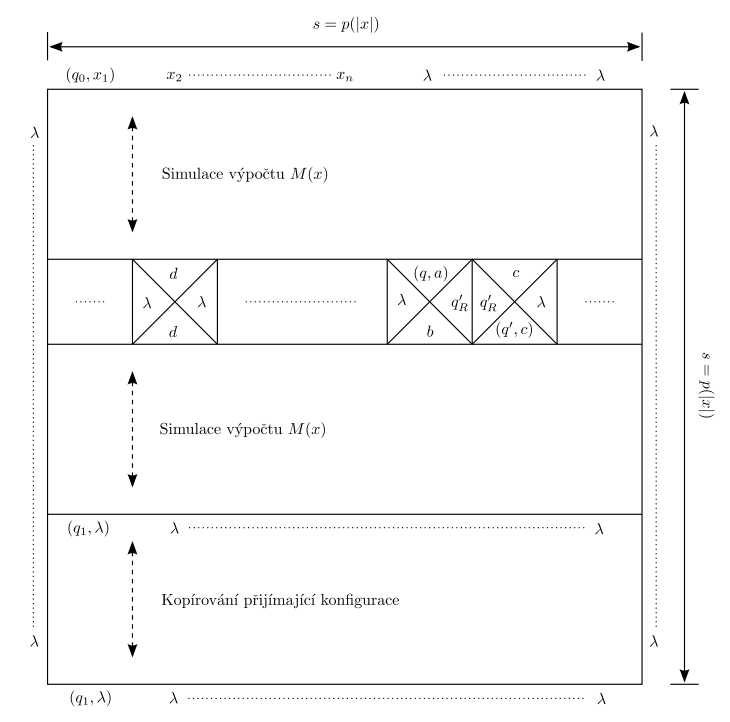
\includegraphics[width=0.8\textwidth]{img/kachl_overview.png}
\end{figure}

Barvy kachlíků tedy budou odpovídat symbolům, které potřebujeme pro zakódování konfigurace, ale budeme potřebovat i pomocné barvy pro přenos informace o stavu o kachlík vlevo nebo vpravo. Položíme tedy
$$ B = \Sigma \cup Q \times \Sigma \cup \{q_L, q_R\ |\ q \in Q\}$$

\begin{itemize}
	\leftskip 20pt
	\setlength{\itemsep}{0pt}
	\item Barva $(q, a)$ v této konfiguraci bude kódovat políčko na pásce, nad kterým se vyskytuje hlava, přičemž $q$ označuje stav, ve kterém se $M$ nachází. Vždy je pouze jedna barva tohoto typu na řádku.
	\item Ostatní políčka konfigurace budou obarvena barvou odpovídající symbolu na daném místě.
	\item Velikost jedné strany čtvercové sítě položíme $s = p(|x|)$.
	\item Boční strany $S$ budou obarveny barvou $\lambda$ (prázdný symbol).
	\item Horní strana $S$ bude obarvena počáteční konfigurací: $[(q_0, x_1), x2, x3, \dots, x_n, \lambda, \dots,\lambda]$, pro vstup $x = x_1x_2x_3\dots x_n$.
	\item Spodní hrana $S$ bude obarvena jednoznačnou přijímající konfigurací: $[(q_1, \lambda), \lambda, \dots, \lambda]$
\end{itemize}

Do typů kachlíků zakódujeme přechodovou funkci Turingova stroje $M$, čímž dosáhneme toho, že správné vykachlíkování řádků 2 až $s$ bude odpovídat výpočtu $M$ nad $x$. Navíc přidáme možnost kopírování přijímající konfigurace tak, abychom ošetřili i případ, kdy výpočet $M$ nad $x$ skončí po méně než $p(|x|)$ krocích.

Použité kachlíky jsou vypsány v tabulce \ref{kachliky}.

\begin{table}[H]
	\centering
	\caption{Kachlíky}
	\label{kachliky}
	\renewcommand{\arraystretch}{1.5}
	\begin{tabular}{| m{0.05\linewidth}  m{0.45\linewidth} | m{0.5\linewidth}| }
		\hline
		(I) & \smallskip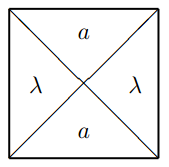
\includegraphics[width=70pt]{img/kachl1.png} 
		& $\forall a \in \Sigma$ kopírování buněk, nad nimiž není hlava\\ 
		(II) & 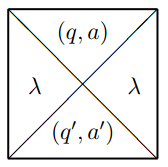
\includegraphics[width=70pt]{img/kachl2.png} 
		& $\forall q \forall a \forall q' \forall a' : (q',a',N) \in \delta(q,a)$\\ 
		(III), (IV) & 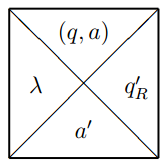
\includegraphics[width=70pt]{img/kachl3.png} 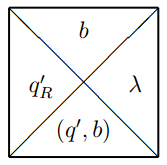
\includegraphics[width=70pt]{img/kachl4.png} 
		& $\forall q \forall a \forall q' \forall a' : (q',a',R) \in \delta(q,a)$\\
		(V), (VI) & 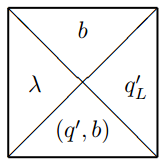
\includegraphics[width=70pt]{img/kachl5.png} 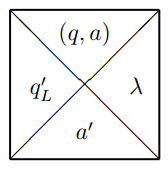
\includegraphics[width=70pt]{img/kachl6.png} 
		& $\forall q \forall a \forall q' \forall a' : (q',a',L) \in \delta(q,a)$\\
		(VII) & 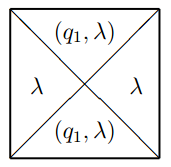
\includegraphics[width=70pt]{img/kachl7.png} 
		& \\ \hline

	\end{tabular}

\end{table}

Funkce f, která bude převádět instanci problému $A$ na instanci problému KACHL provede právě popsanou konstrukci, tj. z popisu $M$ a instance $x$ vytvoří instanci $(B, K, s, S)$, kde množina $K$ obsahuje popsané typy kachlíků a pod $S$ míníme obarvení okrajů sítě. Tuto konstrukci je zřejmě možné provést v polynomiálním čase. Jediné co je v konstrukci závislé na velikosti vstupu je tedy rozměr sítě $s = p(|x|)$ a obarvení horního okraje S počáteční konfigurací.

Zbývá ukázat, že $x \in A \Leftrightarrow $ takto zkonstruovaná instance KACHL má přípustné vykachlíkování:
\begin{description}
	\leftskip 40pt
	\item[$\Rightarrow$:] 
	Předpokládejme nejprve, že $x \in A$ a tedy existuje přijímající výpočet $M(x)$ daný posloupností konfigurací $K_0^x = K_0, \dots, K_t = K_F$. Podle předpokladu platí, že $t \leq p(|x|)$ a délka slova na pásce v každé konfiguraci je rovněž nejvýš $p(|x|)$. Popíšeme, jak s pomocí konfigurací $K_0, \dots, K_t$ obarvit síť $S$. Pro řadu $i = 0$, tj. horní okraj $S$ je vybarvení správně díky konstrukci. Dále indukcí: máme-li validně vybarvenou $i$-tou řadu, vykachlíkujeme $(i + 1)$-ní řadu s odsimulováním příslušné instrukce, která vedla k přechodu z $K_i$ do $K_{i+1}$. Takto se dostaneme k $K_t = K_F$ a poté dokopírujeme KF až na poslední řádek čtvercové sítě $S$. 
	Instrukci lze vždy odsimulovat díky použitým typům kachlíků. 

	\item[$\Leftarrow$] Nechť $\exists$ přípustné vykachlíkování čtvercové sítě $S$. Ukážeme, že řádky barev mezi jednotlivými řádky kachlíků určují posloupnost konfigurací v přijímajícím výpočtu $M$ nad $x$. 
	
	Indukcí dle i: nechť $b_{i,1}, \dots, b_{i,s} \in B$ je posloupnost barev mezi $i$-tým a $(i+1)$-ním řádkem. Musíme ukázat tyto dvě vlastnosti pro každé $i = 0, \dots, s$:
	\begin{enumerate}
		\leftskip 40pt
		\setlength{\itemsep}{0pt}
		\item V posloupnosti $b_{i,1}, \dots, b_{i,s}$ je \textbf{právě jedna barva} typu $(q, a) \in Q \times \Sigma$, ostatní jsou typu $a \in \Sigma$, tj. posloupnost $b_{i,1}, \dots, b_{i,s}$ \textbf{určuje validní konfiguraci} $K_i$.
		\item Platí, že $K_i$ lze z $K_{i-1}$ \textbf{vytvořit pomocí přechodové funkce} $\delta$ pro $i > 0$ a $K_0 = K_0^x$.
	\end{enumerate}

	Obě vlastnosti jsou jistě splněné pro $i = 0$. Předpokládejme nyní, že jsou splněny pro $i \in [0, \dots, s]$ a ukažme, že platí pro $i + 1$. Obě vlastnosti opět jednoduše plynou z toho, jaké kachlíky máme k dispozici. Podle indukčního předpokladu se na řádku barev vyskytuje právě jedna pozice, řekněme $k$, pro kterou platí, že $b_{i,k} = (q, a)$ pro nějaký stav $q \in Q$ a znak $a \in \Sigma$. To znamená, že v $(i + 1)$-ním řádku kachlíků je právě jeden kachlík s horní barvou $(q, a)$, a to na pozici $S[i+1, k]$. Kachlíky nám neumožňují vytvořit barvu $(q, a)$ z ničeho, musí jít o barvu tohoto typu převedenou z předchozího řádku, a to buď kachlíkem (II) a nebo kachlíky (III) a (IV) a nebo kachlíky (V) a (VI).

	Spodní hrana $S$ je obarvena přijímající konfigurací, takže poslední řada barev kachlíků musí
	odpovídat přijímající konfiguraci. 
	
	Dostáváme tedy, že posloupnost konfigurací daných barvami na hranách mezi řádky kachlíků v čtvercové síti $S$ odpovídají přijímajícímu výpočtu $M$ nad vstupem $x$ a jde dokonce o vzájemnou korespondenci, a tedy máme-li přípustné vykachlíkování, znamená to, že $M(x)$ přijme. Z toho plyne, že $x \in A.$
\end{description}


\end{proof}

\section{Pseudopolynomiální algoritmy, silná NP-úplnost.}


\section{Aproximační algoritmy a schémata.}
Pokud nejsme schopni rychle získat optimální řešení NP-úplné úlohy, můžeme slevit ze svých požadavků a pokusit se najít řešení, jež není od toho optimálního příliš vzdáleno. Nejprve si upřesníme pojem optimalizační úlohy:

\textbf{Optimalizační úlohu} definujeme jako trojici $A = (D_A, S_A, \mu_A)$, kde
\begin{itemize}
	\leftskip 20pt
	\setlength{\itemsep}{0pt}
	\item $D_A \subseteq \Sigma^*$ je \textbf{množina instancí}
	\item $S_A(I)$ je \textbf{množina přípustných řešení} pro instanci $I \in D_A$
	\item $\mu_A(I, \sigma)$ přiřazuje instanci $I \in D_A$ a přípustnému řešení  $\sigma \in S_A(I)$ kladné racionální číslo, tzv. \textbf{hodnotu řešení}.
\end{itemize}

Úloha může být $A$ \textbf{maximalizační} resp. \textbf{minimalizační}, pak optimálním řešením instance $I$ je to přípustné řešení $\sigma \in S_A(I)$, jež má \textit{maximální} resp. \textit{minimální} hodnotu $\mu_A(I, \sigma)$.

\textbf{Hodnotu optimálního řešení} označíme pomocí $opt(I)$.

Příklad: Minimalizační úloha \textit{Vrcholového pokrytí (VP)}: 
\begin{itemize}
	\leftskip 20pt
	\setlength{\itemsep}{0pt}
	\item množina instancí $D_{VP}$ = všechny řetězce kódující nějaký graf $G = (V,E)$	
	\item množina přípustných řešení pro instanci $G$, tj. $S_{VP}(G)$ = všechny množiny vrcholů $S \subseteq V$ pokrývající všechny hrany
	\item hodnota řešení S, tj. $\mu_{VP}(G,S) = |S|$, tedy počet vrcholů v množině
\end{itemize}


Algoritmus $R$ nazveme \textbf{aproximačním algoritmem} pro optimalizační úlohu $A$, pokud pro každou instanci $I \in D_A$ je výstupem $R(I)$ přípustné řešení $\sigma \in S_A(I)$ (pokud nějaké existuje).

Je-li $A$ \textit{maximalizační} úloha, pak $\varepsilon \geq 1$ je \textbf{aproximačním poměrem} algoritmu $R$, pokud pro každou instanci $I \in D_A$ platí, že 
$$opt(I) \leq \varepsilon \cdot \mu_A(I, R(I))$$

Je-li $A$ \textit{minimalizační} úloha, pak $\varepsilon \geq 1$ je \textbf{aproximačním poměrem} algoritmu $R$, pokud pro každou instanci $I \in D_A$ platí, že 
$$\mu_A(I, R(I)) \leq \varepsilon \cdot opt(I)$$



\chapter{Datové struktury}
\section{Vyhledávací stromy ((a,b)-stromy, Splay stromy).}
\section{Haldy (regulární, binomiální).}
\section{Hašování, řešení kolizí, univerzální hašování, výběr hašovací funkce.}
\section{Analýza nejhoršího, amortizovaného a očekávaného chování datových struktur.}
\section{Chování a analýza datových struktur na systémech s paměťovou hierarchií.}



\part{Inteligentní agenti}

\chapter{Přírodou inspirované počítání}
\section{Genetické algoritmy, genetické a evoluční programování.}
\subsection{Evoluční algoritmy}
\textbf{Evoluční algoritmy (EA)} je souhrnné označení pro všechny výpočetní metody inspirované evolucí. Historicky se nejdříve paralelně vyvíjely 3 metodiky: genetické algoritmy, evoluční strategie a evoluční programování. Až později došlo k jejich seskupení pod společný zastřešující název: evoluční algoritmy (někdy také evoluční počítání).

EA jsou populační stochastické prohledávací algoritmy. Obecně se hodí spíše označení meta-algoritmus, jelikož pro specifické problémy se vytváří doménově specifické varianty EA s doménově danou reprezentací a vlastními implementacemi evolučních operátorů. Obecně platí \uv{no free lunch theorem} -- tj. neexistuje jeden ultimátní nejlepší algoritmus pro všechny typy problémů.

Základní struktura obecného EA je následující:
\begin{enumerate}
	\leftskip 40pt
	\setlength{\itemsep}{0pt}
	\item vytvoř náhodnou iniciální populaci $P(t=0)$, ohodnoť $P(0)$
	\item dokud není splněna ukončovací podmínka:
	\begin{enumerate}
		\leftskip 40pt
		\setlength{\itemsep}{0pt}
		\item rodičovská selekce podle fitness
		\item křížení s pravděpodobností $p_c$
		\item mutace s pravděpodobností $p_m$
		\item ohodnocení nové populace, environmentální selekce do $P(t+1)$
	\end{enumerate}
\end{enumerate}
\begin{figure}[H]
	\centering
	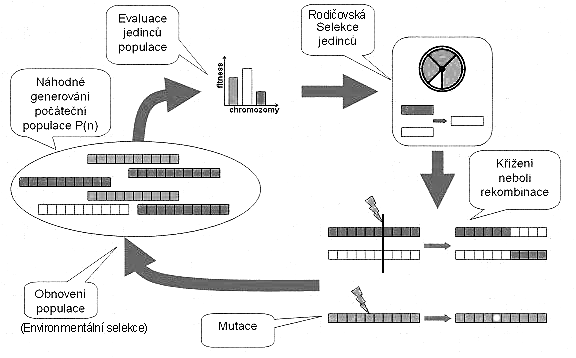
\includegraphics[width=0.8\textwidth]{img/ea.png}
\end{figure}

\subsection{Genetické algoritmy (GA)}
Původní Hollandův GA (dnes označován jako Simple GA, SGA) je nejstarší a nejjednodušší varianta EA, jejímž klíčovým rysem je to, že jedinci jsou \textbf{binární řetězce}. Používá ruletovou selekci (rodičovskou, environmentální se nepoužívá), 1-bodové křížení, bitové mutace (viz níže). V původním Hollandově návrhu je i operátor \textit{inverze}, který obrátí část řetězce, ovšem se zachováním významu bitů. Inverze se ukázala být nevýhodnou.


%TODO GA

\subsection{Genetické programování (GP)}
\begin{wrapfigure}{r}{0.3\textwidth}
\centering
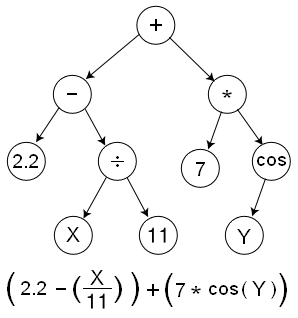
\includegraphics[width=0.25\textwidth]{img/gp.png}
\end{wrapfigure}
Tento pojem označuje genetické algoritmy, v nichž je jedincem v populaci počítačový \textbf{program}. Myšlenkou tedy je, že budeme evolvovat počítačový kód, který za nás bude řešit problémy. Duchovním otcem GP je John Koza. V jeho původní práci jsou programy reprezentovány jako syntaktické stromy, kde listy jsou proměnné a konstanty, vnitřní uzly jsou operace. \textbf{Křížení} je výměna podstromu, \textbf{mutací} se používá několik typů: mutace konstant, výměna uzlu stejné arity, permutace podstromů, záměna neterminálu za terminál apod. \textbf{Fitness} je poměrně jednoduchá: spustit vygenerovaný program na testovacích datech a ohodnotit, nakolik řeší daný problém.

Vylepšení základního principu je použití \textbf{automaticky definovaných funkcí (ADF)}. To jsou samostatné stromy, které mají omezenou množinu terminálů i neterminálů a jsou charakterizovány svou aritou. Volání nějaké ADF je pak novým terminálem, který se může vyskytnout v listech. Celý program pak sestává z hlavního stromu a několika vedlejších stromů ADF. Genetické operace GP pracují buď jen v rámci hlavního programu nebo v rámci ADF.

GP se často potýká s problémem bobtnání (\textbf{bloat}), tj. programy mají tendenci narůstat. V praxi se to řeší restrikcí velikosti či hloubky stromu, a to buď jako penalizující člen ve fitness a nebo jako kontrola (a případná eliminace) nově vznikajících jedinců. Zavádí se taky \textit{anti-bloat} operátory, tedy křížení a mutace, které jedince nezvětšují, případně jej rovnou zmenšují.

Kromě stromů lze použít i jiné struktury. \uv{Cestou dolů} jsou \textbf{lineární GP}, tj. program je lineární sekvence příkazů. To vede k jednodušším operátorům i celkové reprezentaci, rovněž rychlejší emulaci běhu; nicméně je tu velké riziko toho, že vznikne nesmyslný program. \uv{Cestou nahoru} jsou \textbf{grafové GP}, kde program je (často acyklický) graf. Vznikly nejprve jako rozšíření na paralelní programy, později získaly obecnější tvar a dnes se používají např. pro evoluci obvodů či neuronových sítí. Kvůli větší komplexitě reprezentace jsou komplikovanější i genetické operátory.

\subsection{Evoluční programování (EP)}
Evoluční programování je jeden z nejstarších směrů vývoje evolučních algoritmů, dokonce ještě o něco starší než Hollandovy GA (60. léta). Průkopníkem je Lawrence Fogel. Zásadní myšlenkou je vyvinout \uv{umělou inteligence}, konkrétně agenta, který bude umět předpovídat stav prostředí -- jinými slovy bude umět odvodit patřičnou akci v reakci na prostředí, v němž se nachází. Agent je zde reprezentován \textbf{konečným automatem}, prostředí je pak \textbf{sekvence symbolů konečné abecedy}.

Samotná evoluce pak vypadá takto: jedinci v populaci jsou konečné automaty, těm jsou předkládány vstupy. Jejich výstup je vždy porovnán s následujícím vstupem v posloupnosti. Fitness je úspěšnost predikce, přičemž se může měřit různě: vše nebo nic, absolutní chyba, mean square error. Často je do fitness započítána i velikost automatu.

\textit{Každý} automat podstoupí mutaci, která může mít různou \uv{intenzitu} -- od malých, \uv{kosmetických} změn po radikální. Příklady mutací jsou: změna výstupního symbolu, změna následného stavu, přidání stavu, odebrání stavu, změna počátečního stavu, \dots Noví jedinci jsou ohodnoceni a poté je vybráno (z nových i starých najednou) $N$ jedinců do nové populace. Výběr probíhá buď turnajem, nebo deterministicky (tj. vezme se $N$ nejlepších jedinců. (Pozn.: V původním algoritmu není nijak omezeno, kolik potomků může být vygenerováno z jednoho rodiče, ani že velikost populace musí zůstávat konstantní.)

\textbf{Křížení neexistuje (!)}. 

V dnešní době se EP vyvinulo do obecnější podoby. Zakódování jedinců je velmi benevolentní a mělo by být přirozené pro daný problém (často genotyp = fenotyp). Používá se více \uv{chytrých mutací}, které jsou těsně přizpůsobeny problému a dané reprezentaci. Křížení se typicky nepoužívá. Rodičovská selekce je prostá: každý jedinec se vybere právě jednou. Environmentální selekce je turnajová na spojené populaci rodičů a potomků.

Jelikož se EP vyvíjelo paralelně s GA i ES, jsou mezi nimi nevyhnutelně mnohé podobnosti. Pojďme si tyto metody porovnat.

\subsubsection{EP vs. GA}
V GA jsou jedinci sekvence symbolů abecedy, původně pouze binární, dnes už vcelku libovolné. V EP není žádné omezení na podobu reprezentace a typicky je přizpůsobena problému (jedinec může být např. neuronová síť). 

Mutace funguje rovněž trochu jinak. V EP máme škálu mutací od malých změn až po radikální zásahy, přičemž pravděpodobnost aplikace mutace je nepřímo úměrná její závažnosti. Celková závažnost mutací se rovněž může snižovat v průběhu konvergence k optimálnímu řešení.

Zjevným rozdílem je rovněž absence křížení u EP.

\subsubsection{EP vs. ES}
Pokud je jedincem v EP posloupnost reálných čísel, začínají být velice podobné evolučním strategiím. EP dokonce také mohou být \textit{self-adaptive}, tj. jedinec nese kromě genotypu i parametry ovlivňující evoluci, konkrétně míru závažnosti mutací (rozptyl gaussovské mutace).

Existují však rozdíly: EP používá turnajovou selekci, ES deterministicky odstraňuje dané množství nejhorších řešení. Druhým rozdílem je absence křížení u EP, zatímco ES je často implementuje. 

\subsubsection{Význam křížení}
Malá odbočka: trpí EP tím, že nemá křížení? Pomáhá vlastně křížení, nebo stačí mutace? Jones (1995) provedl tzv. \uv{headless chicken epxeriment}: porovnával klasické GA a GA, kde je klasické křížení nahrazeno \uv{náhodným křížením}. To funguje tak, že se dva vybraní jedinci nezkříží mezi sebou, namísto toho se pro každého z nich vygeneruje partner jako náhodná sekvence z domény (tj. například náhodný binární vektor správné délky). Pak se provede jednobodové křížení a od každého rodiče se vybere jeden potomek. Jones označil tento operátor jako \textit{headless chicken} -- stejně jako bezhlavé kuře pobíhající po dvorku není doopravdy kuře (protože mu něco důležitého chybí), tak ani toto \uv{náhodné křížení} není vlastně křížení, protože při něm vůbec nedochází ke kontaktu mezi jedinci. Jedná se ve skutečnosti o jakousi makromutaci.

Pointou experimentu bylo porovnat výkonnost obou variant a určit, nakolik opravdové křížení skutečně pomáhá. Závěrem bylo konstatování, že pokud má problém jasně definované stavební bloky, pak křížení skutečně pomáhá (především na začátku evoluce), zatímco pokud nejsou bloky zřejmé, pak křížení příliš nepomáhá (výkon obou variant byl srovnatelný).

\section{Teorie schémat, pravděpodobnostní modely jednoduchého genetického algoritmu.}
\subsection{Schémata}
\textbf{Schéma} v kontextu genetických algoritmů (tj. jedinec je slovo v abecedě \{0,1\}) je reprezentace množiny jedinců jako slova v abecedě \{0,1,*\}, kde * označuje libovolný symbol (\uv{žolík}). Například schéma 0*11* reprezentuje množinu jedinců \{00110, 00111, 01110, 01111\}. Platí následující:
\begin{itemize}
	\leftskip 20pt
	\setlength{\itemsep}{0pt}
	\item schéma s $r$ * reprezentuje $2^r$ jedinců
	\item jedinec délky $m$ je reprezentován $2^m$ schématy
	\item je $3^m$ schémat délky $m$
	\item v populaci velikosti $n$ je $2^m$ až $n\cdot2^m$ schémat
\end{itemize}
Pro schéma S lze definovat následující vlastnosti:
\begin{description}
	\leftskip 20pt
	\setlength{\itemsep}{0pt}
	\item[Řád schématu o(S):] počet pevných pozic (0 a 1) 
	\item[Definující délka d(S):] vzdálenost mezi první a poslední pevnou pozicí
	\item[Fitness F(S)] průměrná fitness odpovídajících jedinců v populaci
\end{description}

\noindent\textbf{Věta o schématech (VoS):} \textit{Krátká schémata s nadprůměrnou fitness a malým řádem se v populaci během GA exponenciálně množí.}


\begin{proof} Budeme zkoumat, co se děje s konkrétním schématem $S$ během selekce, křížení a mutace.

Nechť $P(t)$ je populace v čase $t$, $n$ je velikost populace, $m$ je délka jedinců v populaci, $C(S,t)$ je četnost schématu $S$ v populaci $P(t)$ (tj. počet jedinců v $P(t)$ reprezentovaných $S$). Budeme odhadovat $P(S, t+1)$.

\textit{Selekce:} Schéma $S$ má pravděpodobnost vybrání
$$p_s(S) = \frac{F(S)}{\sum\limits_{u \in P(t)}F(u)}$$
Tedy 
$$C(S,t+1) = C(S,t) \cdot n \cdot p_s(S)$$
neboť provádím $n$ výběrů do nové populace pomocí ruletové selekce, přičemž na ruletě zabírají jedinci odpovídající schématu $S$ právě $C(S,t) \cdot p_s(S)$ procent místa. Ekvivalentně lze psát
$$C(S,t+1) = C(S,t) \cdot \frac{F(S)}{\frac{\sum_{u \in P(t)}F(u)}{n}} = C(S,t) \cdot \frac{F(S)}{F_{avg}(t)}$$
kde $F_avg(t)$ označuje průměrnou fitness v populaci $P(t)$. 

Představme si, že schéma $S$ je nadprůměrné o $\varepsilon$\,\%, tj. $F(S) = F_{avg}(t) + \varepsilon\cdot F_{avg}(t)$. Pak 
$$C(S,t+1) = C(S,t)(1+\varepsilon)$$
$$C(S,t+1) = C(S,0)(1+\varepsilon)^t$$
Tedy četnost nadprůměrných schémat roste geometrickou řadou.

\textit{Křížení:} Předpokládáme klasické jednobodové křížení. Pravděpodobnost, že schéma $S$ křížení nepřežije, je 
$$p_{death}(S) = \frac{d(S)}{m-1}$$
a tedy pravděpodobnost přežití je 
$$p_{surv}(S) \geq 1 - p_c \cdot \frac{d(S)}{m-1}$$
kde $p_c$ je pravděpodobnost křížení. Všimněte si nerovnosti: je totiž šance, že i když se bod křížení \uv{trefí} dovnitř schématu, tak část doplněná s druhého rodiče bude pořád odpovídat schématu a celkově tedy schéma přežije. Zjevné je to například při křížení dvou totožných jedinců (tam schéma přežije vždy).

\textit{Mutace:} Pravděpodobnost změny jednoho bitu je $p_m$, pravděpodobnost přežití schématu je tedy 
$$p_{surv}(S) = (1-p_m)^{o(S)}$$
$$p_{surv}(S) \approx 1 - p_m \cdot o(S)$$
Poslední aproximace funguje pro $p_m \ll 1$.

Dohromady tedy dostáváme:
$$C(S,t+1) \geq C(S,t) \cdot \frac{F(S)}{F_{avg}(t)} \cdot \left(1 - p_c \cdot \frac{d(S)}{m-1} - p_m \cdot o(S)\right)$$
\end{proof}

\textbf{Hypotéza o stavebních blocích (HoSB)} GA hledá suboptimální řešení problému rekombinací krátkých, nadprůměrných s malým řádem schémat (\uv{building blocks}).

\subsubsection{Důsledky VoS}
GA pracuje s $n$ jedinci, ale implicitně vyvíjí mnohem více schémat: $2^m$ až $n\,2^m$ (implicitní paralelismus). Holland tvrdí, že za splnění jistých předpokladů ($n = 2^m$, schémata zůstávají nadprůměrná, \dots) platí, že počet schémat, kterým se v GA dostává exponenciálního růstu je úměrný $n^3$. 

GA také optimálně řeší problém explorace a exploatace, což lze ukázat na analogii s tzv. \textbf{2-rukým banditou}: \textit{Mám N mincí, ruce bandity (= hrací automat) vyplácí se střední hodnotou $m_1$ resp. $m_2$ a rozptylem $s_1$ resp. $s_2$, cílem je maximalizovat zisk. Analytickým řešením je alokovat exponenciálně více pokusů pro právě vyhrávající ruku.} GA rovněž alokuje exponenciálně mnoho nadějným schématům. Nejdříve se myslelo, že GA hraje $3^m$-rukého banditu, tj. všechna schémata jsou konkurenční ruce. Ve skutečnosti se hraje více her, v nichž schémata soutěží o konfliktní pevné pozice: schémata řádu $k$ soutěží právě o těch $k$ pozic -- hrají spolu $2^k$-rukého banditu. To stále není úplně přesné, protože na rozdíl od bandity, kde jsou ruce nezávislé, nesampluje GA schémata nezávisle.

Problémem také je, že GA často neodhadne správně skutečnou fitness schémat. Např. je-li F(111*\dots*)~= 2, F(0*\dots*) = 1 a jinak F(x) = 0, pak platí F(1*\dots*) = $\frac{1}{2}$, F(0*\dots*) = 1. Jenže GA odhadne F(1*\dots*) $\approx$ 2, protože 111*\dots* v populaci převáží. Tomuto se říká \textit{kolaterální konverence}, tj. jakmile se někam začne konvergovat, už nejsou schémata samplována rovnoměrně a fitness se neodhadne správně. Podobným problémem je velký rozptyl fitness (např. 1*\dots* z předchozího příkladu). GA bude nejspíše konvergovat tam, kde je fitness větší $\rightarrow$ chybný odhad statické fitness.


\subsection{Pravděpodobnostní modely}
Od 90. let se objevují snahy přesně modelovat chování GA, konkrétně: jak přesně vypadají populace, zobrazení přechodu k další populaci, vlastnosti tohoto zobrazení, asymptotické chování jednoduchého GA. Existují modely pro konečné i nekonečné populace.

\subsubsection{Ještě jednodušší jednoduchý GA (JJJGA)}
Pro jednodušší tvorbu modelů byl původní jednoduchý GA ještě o něco zjednodušen a formalizován takto:
\begin{itemize}
	\leftskip 20pt
	\setlength{\itemsep}{0pt}
	\item inicializuj náhodnou počáteční populaci binárních řetězců $x$ délky $l$
	\item dokud nenajdeš dost dobré $x$:
	\begin{itemize}
		\leftskip 40pt
		\setlength{\itemsep}{0pt}
		\item dokud nenaplníš novou populaci:
		\begin{itemize}
			\leftskip 40pt
			\setlength{\itemsep}{0pt}
			\item vyber selekcí 2 jedince, zkřiž je s pravděpodobností $p_c$, jednoho potomka zahoď
			\item mutuj každý bit nového řetězce s pravděpodobností $p_m$
			\item vlož do nové populace
		\end{itemize}
	\end{itemize}
\end{itemize}

\subsubsection{Analýza}
Každý jedinec je tedy binární řetězec délky $l$, což lze chápat jako binární zápis nějakého čísla [0, \dots, $2^l-1$] (např. 00000111 je 7). Populace v čase $t$ je reprezentována dvěma vektory $p(t)$ a $s(t)$, oba délky $2^l$. Číslo $p_i(t)$ vyjadřuje, kolik procent populace zabírá řetězec $i$; číslo $s_i(t)$ vyjadřuje pravděpodobnost selekce řetězce $i$.

Dále definujeme matici $F$ takto: $F(i,i) = f(i); F(i,j) = 0$ pro $i \neq j$. Hodnota $f(i)$ je fitness jedince $i$. Pak můžeme definovat vztah vektorů $s(t)$ a $p(t)$ jako
$$s(t) = \frac{F \cdot p(t)}{\sum\limits_{j=0}^{2^l-1} F(j,j) \cdot p_j(t)}$$

Naším ideálem je definovat matici G, která realizuje jeden krok JJGA, tj. $p(t+1) = G \cdot p(t)$, nebo obdobně $s(t+1) = G \cdot s(t)$. Toto zobrazení bude fungovat jako složení dvou dílčích zobrazení: matice F (fitness) a matice M (mutace a křížení). 

Nejprve uvažme $G=F$ (tj. nemáme žádné genetické operátory). Platí $E(p(t+1)) = s(t)$, kde $E$ je střední hodnota. Pak díky $s(t+1) \sim F \cdot p(t+1)$ (liší se jen o multiplikativní odchylku) můžeme psát $E(s(t+1)) \sim F \cdot s(t)$. V případě konečné populace nám výběrové chyby mohou způsobit odchylku od $E()$, obecně čím větší populace, tím menší odchylka. U nekonečné populace by to bylo přesné.

Nyní se podívejme na situaci $G = M$, tedy neřešíme selekci. Zde využijeme pomocnou veličinu $r(i,j,k)$, která udává pravděpodobnost, že z $i$ a $j$ vznikne $k$. Když tuto veličinu známe, pak lze vyjádřit 
$$E(p_k(t+1)) = \sum\limits_{i=0}^{2^l-1} \sum\limits_{j=0}^{2^l-1} s_i(t) \cdot s_j(t) \cdot r(i,j,k)$$
Funkci $r(i,j,k)$ lze analyticky spočíst.\footnote{\url{http://ktiml.mff.cuni.cz/~neruda/eva2-13.pdf}}

Závěr: JJGA pracující prostřednictvím $G$ je dynamický systém, $p(t)$ či $s(t)$ jsou body (trajektorie). Neznáme jeho pevné body, můžeme však vyjádřit pevné body jednotlivých zobrazení: Pevné body F jsou populace se stejnou fitness, stabilní pevný bod F je maximální stejná fitness. (Jediný) pevný bod M: stejné pravděpodobnosti $s$ (resp. stejné zastoupení jedinců $p$). Kombinace míchání M a ostření F odpovídá fenoménu \textit{punctuated equilibria} (známe z biologie).

\subsubsection{Konečné populace}
Pro konečné populace lze definovat GA jako \textit{markovovský řetězec}, tj. stochastický proces v systému se stavy a přechody mezi stavy s definovanými pravděpodobnostmi. Pravděpodobnost přechodu závisí vždy pouze na předchozím stavu. Jeden stav systému je jedna konkrétní populace. Populací o $n$ jedincích délky $l$ je $N = \binom{n+2^l-1}{2^l-1}$, matice pravděpodobností přechodů je $N\times N$, podrobnější rozbor opět v Nerudových slajdech.

Dokázala se korespondence ideálního JJGA s nekonečnou populací a modelu s konečnou populací (pro $n \rightarrow \infty$).






\section{Evoluční strategie, diferenciální evoluce, koevoluce, otevřená evoluce.} 
\subsection{Evoluční strategie}
\textbf{Evoluční strategie (ES)} je metoda pro optimalizaci reálných funkcí, která je výjimečná tím, že jako první používala \textit{self-adaptation}, tj. parametry evoluce byly součástí jedince -- šlo tedy o \uv{evoluci evoluce}. Evolvovaný jedinec se tedy skládá z \textbf{genetických parametrů} ovlivňujících chování a \textbf{strategických parametrů} ovlivňující evoluci.

Vznikly v 60. letech, autoři \textbf{Rechenberg a Schwefel.} ES jsou jedna z větví evolučních algoritmů (anglicky se jako \uv{umbrella term} používá buď \textit{Evolutionary Algorithms} nebo \textit{Evolutionary Computation}), nicméně nevyčlenily se v průběhu, jak by se dalo čekat. ES se vyvíjely paralelně s GA a EP (evolučním programováním), až později došlo k seskupení těchto tří metod pod jeden společný obor.

\subsubsection{Notace}
\begin{description}
	\leftskip 20pt
	\setlength{\itemsep}{0pt}
	\item[\textit{M}] počet jedinců v populaci
	\item[\textit{L}] počet vznikajících potomků
	\item[\textit{R}] počet rodičů každého nového jedince
\end{description}
Doporučení: $M > 1$, $L > M$ aby se vytvořily různé selekce (např. $L \approx 7 \cdot M$)

\subsubsection{Varianty}
\begin{description}
	\leftskip 20pt
	\setlength{\itemsep}{0pt}
	\item[\textit{(M+L)} ES] -- M jedinců do nové populace je vybráno z M+L starých i nových jedinců
	\item[\textit{(M,L)} ES] -- M nových jedinců je vybráno jen z L nových potomků (tato varianta se ukázala být robustnější vůči uvíznutí v lokálních extrémech)
\end{description}

\subsubsection{Kódování, genetické operátory}
Jedinec je tvaru $C(i) = [G_n(i), S_k(i)], k \in \{1, n, 2n\}$, tedy první část je samotný genotyp, druhá část jsou parametry evoluce, konkrétně \textbf{hodnoty standardních odchylek floating point mutací}. Podle hodnoty $k$ rozlišujeme 3 varianty:
\begin{description}
	\leftskip 20pt
	\setlength{\itemsep}{0pt}
	\item[k=1]: jedna společná odchylka pro všechny parametry
	\item[k=n]: nekorelované mutace; geometricky se mutuje po elipse rovnoběžné s osami
	\item[k=2n]: korelované mutace, odpovídají mutování z n-rozměrného normálního rozdělení. 
	Pro uložení korelační matice stačí n-rozměrný vektor (???). Tato matice odpovídá matici rotace (tj. elipsa se natočí v optimálním směru).
\end{description}

\begin{figure}[h]
	\centering
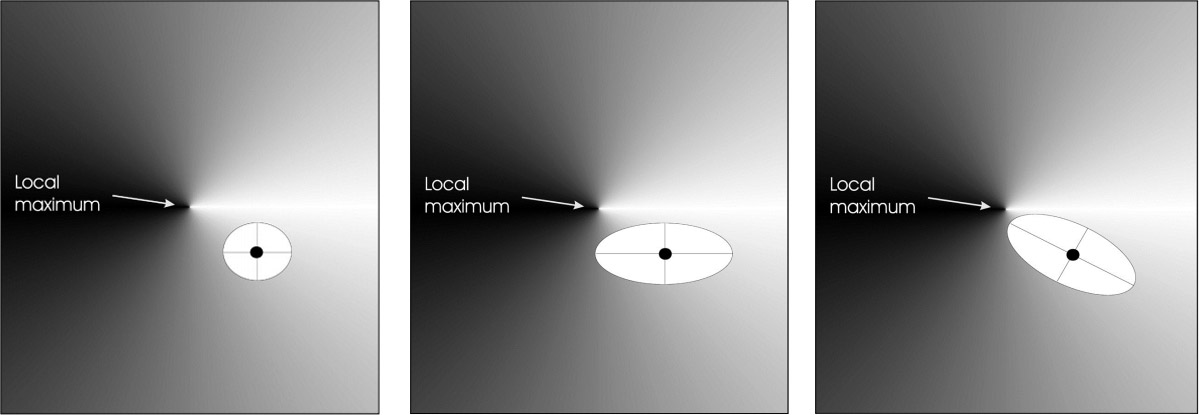
\includegraphics[width=0.7\textwidth]{img/ES_varianty_k.jpg}
\end{figure}

\textbf{Populační cyklus} vypadá takto:
\medskip

\begin{minipage}{\linewidth}
	\begin{lstlisting}[frame=single]
n=0, randomly init population P[n] of size M
evaluate fitness of individuals in P[n]
while not good enough:
	repeat L times:
		choose R parents
		crossover, mutate, evaluate new individual
	choose M new individuals (by the type of ES)
	n++
	\end{lstlisting}
\end{minipage}

Nový jedinec je akceptován pouze tehdy, je-li lepší než rodič -- pak rodiče nahradí.

\textbf{Mutace} jedince probíhá takto: \textit{genetické} parametry (genotyp) jsou změněny přičtením náhodného čísla s norm. rozdělení s příslušnou odchylkou (a případně i rotací). \textit{Strategické} parametry = odchylky jsou zvětšeny nebo zmenšeny podle \uv{pravidla $1/5$}, což heuristika, která říká, že nejlepší je, když má mutace úspěšnost 20\,\% (tzn. při menší zvyš odchylku, při větší sniž). V případě varianty s rotacemi jsou mezi strategickými parametry také hodnoty rotací -- ty se mutují jednoduše přičtením náhodného čísla z N(0,1).

\textbf{Křížení} je uniformní, typicky více rodičů. Podle velikosti R mluvíme o lokálním (R=2) nebo globálním (R=M). Může být diskrétní (použij hodnotu náhodně vybraného rodiče) nebo aritmetické (průměr).

\subsubsection{CMA-ES}
Dnes nejkomplexnější verzí je \textbf{CMA-ES} (Correlation Matrix Adaptation ES). Udržuje se korelační matice proměnných, která se inkrementálně aktualizuje po každém kroku metodou maximum-likelihood.

\subsection{Diferenciální evoluce}
Alternativní algoritmus spojité optimalizace, který funguje dobře i pro funkce které jsou nediferencovatelné, nespojité, zašuměné, neseparabilní nebo vysoce podmíněné. Každý jedinec prochází opakovaně cyklem \textbf{mutace} $\rightarrow$ \textbf{křížení} $\rightarrow$ \textbf{selekce}. Během mutace dochází k posunu \uv{podle ostatních}, tj. jedinec se posouvá ve směru populace. DE je také invariantní vůči rotaci či škálování prohledávaného prostoru.
\begin{figure}[H]
	\centering
	\includegraphics[width=0.7\textwidth]{img/DE_scheme.png}
\end{figure}

\subsubsection{Mutace}
V populaci $p$ zvolíme pro jedince $x_{i,p}$ tři různé jedince: $x_{a,p}$, $x_{b,p}$ a $x_{c,p}$. Definujeme donora: $$v_{i,p+1} = x_{a,p} + F \cdot (x_{b,p} - x_{c,p})$$ kde $F \in \langle 0; 2 \rangle$ je parametr mutace.
\subsubsection{Křížení}
Uniformní křížení původního jedince s donorem. Parametr $C$ určuje pravděpodobnost změny, $rand_{ij} \in \langle0,1\rangle$ je pseudonáhodné číslo. Číslo $I_{rand}$ je náhodný index z $\langle 1,2,...D\rangle$, kde $D$ je délka jedince. Pak vytvoříme pokusný vektor $u_{i,p+1}$ jako:
$$u_{i,p+1}[j] = v_{i,p+1}[j] \leftrightarrow rand_{ji} \leq C \lor j = I_{rand}$$
$$u_{i,p+1}[j] = x_{i,p}[j] \leftrightarrow rand_{ji} > C \land j \neq I_{rand}$$

Díky $I_{rand}$ je zajištěno, že ve výsledku bude aspoň jeden prvek z donora.

\subsubsection{Selekce}
Jako nový jedinec $x_{i,p+1}$ se vezme lepší (dle fitness) z dvojice $x_{i,p}$, $u_{i,p+1}$.

\subsection{Koevoluce}
Situace, kdy se dva či více druhů vyvíjí závisle na sobě, tj. fitness jedince není závislá pouze na prostředí, ale především na interakci s jinými jedinci (tzv. \textit{kontextová fitness}). Rozlišujeme koevoluci \textbf{kooperativní} a \textbf{kompetitivní}. Typickým modelem kompetitivní koevoluce je tzv. \textbf{dravec-kořist} (predator-prey). Kompetitivně lze rovněž vyvíjet strategie pro nejrůznější hry - např. dáma apod.

%TODO koevoluce

\subsection{Otevřená evoluce}
Evoluce bez konce, tj. neexistuje ukončovací podmínka ani optimální řešení, neboť fitness funkce je \textit{dynamická}. Často je dynamické i kódování jedince -- např. pokud u neuroevoluce mohou síti ubývat a přibývat neurony či synapse. 

Míra změn fitness může být různá: 
\begin{description}
	\leftskip 30pt
	\setlength{\itemsep}{0pt}
	\item[malé změny] robot se opotřebuje, v chemické továrně se trochu změní suroviny apod.
	\item[výrazné morfologické změny] vrcholy zanikají, nové vznikají, \uv{emerging markets}
	\item[cyklické změny] roční období, spotřeba elektřiny, \dots
	\item[katastrofické změny] bouchla elektrárna, nehoda na dálnici, \dots
\end{description}

Byly navrženy různé postupy pro vyrovnání se s dynamickou fitness. Například \textit{vyvolaná hypermutace} (při snížení fitness), \textit{náhodná migrace} (při snížení fitness se generují noví náhodní jedinci) a obecně metody vedoucí k udržení diverzity populace: zmenšení selekčního tlaku, crowding, niching, subpopulace, dynamické druhy (které se množí jen mezi sebou).

Dynamická fitness je vyvolaná i kompetitivní koevolucí, a tedy evoluční souboje typ lovec-kořist lze označit za otevřenou evoluci.


%TODO otevřená evoluce


\section{Rojové optimalizační algoritmy.}
\subsection{Optimalizace hejnem částic}
Anglicky \textit{particle swarm optimization} -- jedná se o populační prohledávací algoritmus inspirovaný hejny ptáků/hmyzu/ryb. Jedinec se nazývá \textbf{částice} a jde typicky o vektor reálných čísel. Neexistují křížení ani mutace, jak je známe.

\subsubsection{Algorimus}
\begin{minipage}{\linewidth}
	\begin{lstlisting}[frame=single, escapeinside={\%*}{*)}]
init each particle
while not (max iterations or minimum error)
	foreach particle p:
		f = fitness(p)
		if f > p.pBest
			p.pBest = f
	gBest = max(p.pBest for each particle p)			
	foreach particle p:
		p.v = p.v + 
			+ c1 * rand(0,1) * (pBest - p.position) 
			+ c2 * rand(0,1) * (gBest - p.position) 
		p.position += p.v		
	\end{lstlisting}
\end{minipage}

Každá částice má rychlostní vektor $v$, který se aktualizuje podle nejlepší pozice částice v historii (řádek 10) a nejlepší globální pozice v historii (řádek 11). Učicí konstanty c1,c2 se často nastavují na c1 = c2 = 2. \\
\textit{Pozn. celé to asi může být v jednom for cyklu s tím, že gBest se aktualizuje průběžně a ne po "generacích".}

PSO jsou podobné GA -- stochastický model, fitness pro ohodnocení, náhodná iniciální konfigurace atd. -- ale současně se v mnohém liší: neexistují genetické operace, částice mají paměť a výměna informací probíhá pouze od nejlepších částic ostatním. 

PSO nepoužívají gradient pro optimalizaci, což znamená, že optimalizovaná funkce nemusí být diferencovatelná.


\subsection{Další rojové optimalizační algoritmy}
Obecně se definuje \textbf{Swarm Intelligence (SI)} jako \textit{“The emergent collective intelligence of groups of simple agents"}. Dvě základní vlastnosti jsou sebeorganizace a dělba práce. Kromě PSO sem lze zařadit ještě Ant Colony Optimization (ACO), Artificial Bee Colony (ABC), Glowworm Swarm Optimization, Cuckoo Search Algorithms a v jistém směru sem spadá i diferenciální evoluce (jelikož je population-based). Kromě DE se tyto algoritmy (a mnohé další, třeba i simlated annealing)  označují také nálepkou \textit{metaphor-based metaheuristics}, a to díky tomu, že jsou typicky insipirované nějakou reálnou skutečností (chování roje, chování mravenců, zpracování kovů apod.). Tyto se staly terčem kritiky pro nedostatek inovace a efektivity, kterou schovávají právě za poutavou metaforou (\url{https://en.wikipedia.org/wiki/List_of_metaphor-based_metaheuristics}).

\subsubsection{Ant Colony Optimization (ACO)}
Systém inspirovaný chování mravenců při hledání potravy, konkrétně použitím feromonů. V podstatě jde o techniku nalezení nejlepší cesty v grafu. Agent (mravenec) se pohybuje v grafu a zanechává za sebou feromonovou stopu. Pohyb se řídí rovnicí:
$$p^k_{ij}(t) = \frac{([\tau_{ij}(t)]^\alpha \cdot [\eta_{ij}]^\beta)}{(\sum\limits_{n \in J_k}[\tau_{in}(t)]^\alpha \cdot [\eta_{in}]^\beta)}$$

$p^k_{ij}(t)$ je pravděpodobnost přechodu mravence $k$ z uzlu $i$ do uzlu $j$ v čase $t$, $J_k$ jsou uzly, kam má mravenec $k$ povoleno jít, $\eta_{ij}$ symbolizuje \uv{viditelnost} mezi $i$ a $j$ a $\tau_{ij}(t)$ reprezentuje množství nevypařeného feromonu mezi $i$ a $j$ v čase $t$. Parametry $\alpha$ a $\beta$ kontrolují, nakolik prohledávání závisí na feromonech. Každý mravenec $k$ má také tabu list navštívených uzlů, aby nenavštívil nějaký dvakrát.

Umístění feromonů se řídí rovnicí:
\[
\Delta\tau^k_{ij} = 
\begin{cases}
	\frac{Q}{L_k}(t) 	& \quad \text{leží-li hrana $ij$ na cestě mravence $k$} \\
	0 					& \quad \text{jinak}\\
\end{cases}
\]

$Q$ je konstanta, $L_k$ je cena cesty (její délka), $k$ je mravenec, $t$ je čas (iterace).

Feromony se časem vypařují. Celková změna feromonu na hraně $ij$ je tedy:
$$\tau_{ij}(t+1) = (1-p)\tau_{ij}(t) + \sum_{k=1}^m [\Delta\tau^k_{ij}(t)]$$
kde $m$ je počet mravenců a $p$ je míra vypařování. To je důležitý parametr algoritmu, který ovlivňuje poměr mezi explorací a exploatací.

Mírně vylepšená varianta ACO je Ant Colony System (ACS).

Dobrý přehled dalších algoritmů (např Artificial Bee Colony) lze nalézt na \url{http://journals.plos.org/plosone/article?id=10.1371/journal.pone.0122827}






\section{Memetické algoritmy, hill climbing, simulované žíhání.}
\textbf{Memetické algoritmy} jsou EA obohacené o lokální prohledávání uvnitř cyklu. Základní princip je ten, že evolucí vyvinutý jedinec ještě před ohodnocením podstoupí proceduru lokálního prohledávání -- to může být např. hill climbing, simulované žíhání nebo backpropagation u ANN). 

Inspirováno \textbf{mémy} (angl. \textit{meme} (čti /mi:m/)), což jsou ideje/myšlenky šířící se ve společnosti, které mohou podstoupit mutaci či selekci, stejně jedinci v klasické evoluci. 

Alternativně jsou MA označovány jako \textit{Baldwinian EA}, \textit{Lamarckian EA} nebo jako \textit{genetic local search}.

\subsubsection{Algoritmus}
\begin{minipage}{\linewidth}
	\begin{lstlisting}[frame=single, escapeinside={\%*}{*)}]
t = 0, initialize P[0]
P[0].localSearch()
evaluate(P[0])
while notTerminated do
	P[t] = selectIndividuals()
	mutate(P[t])
	P[t].localSearch()
	evaluate(P[t])
	P[t+1] = buildNextGen(P[t])
	t++

	\end{lstlisting}
\end{minipage}

\subsubsection{Existují dva přístupy, co dělat s výsledkem:}
\begin{description}
	\leftskip 20pt
	\setlength{\itemsep}{0pt}
	\item[Lamarckismus] Když prohledáváním najdu lepšího jedince, vezmu ho (to je ovšem darwinisticky nekorektní, změnil jsem genotyp na základě fenotypu).
	\item[Baldwinismus] Když lokálním prohledáváním najdu lepšího jedince, vezmu jen jeho fitness (ale neměním genotyp).
\end{description}


\subsubsection{Hill climbing}
Nejjednodušší informovaná metoda lokálního prohledávání stavového prostoru. Vstupem je uzel, ze kterého se má prohledávání zahájit. Nejprve je uzel expandován - jsou vygenerovány jeho sousední uzly a tyto uzly jsou ohodnoceny. Algoritmus vybere z nich nejlépe ohodnocený uzel a ten je nadále expandován. 

Algoritmus tak expanduje uzly se stále vyšším ohodnocením, dokud nenarazí na uzel po jehož expanzi mají všechny jeho sousední uzly horší ohodnocení. Algoritmus nemá paměť, navštívené uzly okamžitě zapomíná.

\medskip\textbf{Varianty:}
\begin{description}
	\leftskip 30pt
	\setlength{\itemsep}{0pt}
	\item[first choice HC vs. steepest ascent HC] First choide HC vezme prvního lepšího souseda, steepest zkusí všechny a vezme nejlepšího.
	\item[stochastic HC] Ze zlepšujících sousedů vybere náhodně podle míry zlepšení.
	\item[random restart HC (or shotgun HC)] Náhodné restarty v různých místech, částečně řeší problém uvíznutí v lokálním optimu.
\end{description}


\subsubsection{Simulované žíhání}
	\setlength\intextsep{0pt}
\begin{wrapfigure}{r}{0.35\textwidth}
	\centering

	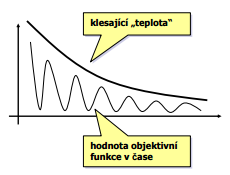
\includegraphics[width=0.3\textwidth]{img/simulated_annealing.png}
\end{wrapfigure}
Lokální prohledávání kombinující HC a náhodnou procházku. Algoritmus náhodně volí stav okolí a vydá se do něj pokud:
\begin{itemize}
	\leftskip 20pt
	\setlength{\itemsep}{0pt}
	\item je lepší než aktuální stav
	\item je horší, ale zhoršení je povoleno s určitou mírou pravděpodobnosti odvozenou od aktuální \textbf{teploty}; teplota se přitom postupně snižuje podle „ochlazovacího“ schématu
\end{itemize}


\subsubsection{Algoritmus}
\begin{minipage}{\linewidth}
\begin{lstlisting}[frame=single, escapeinside={\%*}{*)}]
	current = init()
	for t = 1 to %*$\infty$*)
		T = schedule(t)
		if T = 0 then 
			return current
		next = randomNeighbor(current)
		%*$\Delta$E*) = f(next) - f(current)
		if (%*$\Delta$E*) > 0) or (%*$e^{\Delta{}E/T} < $*) rand(0,1))
			current = next
\end{lstlisting}
\end{minipage}






\section{Aplikace evolučních algoritmů (evoluce expertních systému, neuroevoluce, řešení kombinatorických úloh, vícekriteriální optimalizace).}
\subsection{Evoluce expertních systémů}
Expertní systémy jsou modely z oblasti \textit{strojového učení}, jejichž základní charakteristikou je, že pro výpočet svého výstupu používají pravidla IF: THEN. Zastupují tedy větev strojového učení založenou na \textit{formální logice} (druhá, protikladná větev, reprezentovaná především neuronovými sítěmi, je založena na \textit{konekcionismu}, tj. modeluje biologické fungování mozku, nikoli logické). Expertní systémy, které se učí pomocí simulované evoluce, se nazývají \textbf{learning classifier systems (LCS)}. Existují dvě základní paradigmata: \textit{michiganský přístup} (jedinec je pravidlo) a \textit{pittsburghský přístup} (jedinec je množina pravidel).

\begin{wrapfigure}{r}{0.45\textwidth}
\centering
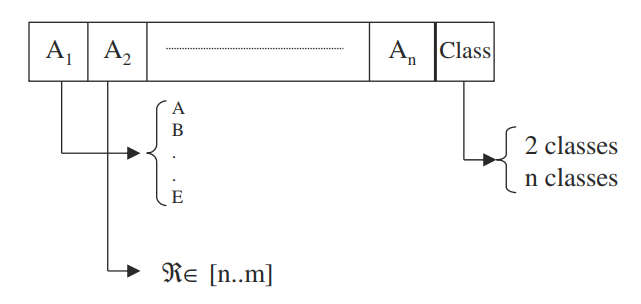
\includegraphics[width=0.4\textwidth]{img/classification_instance.png}
\end{wrapfigure}
Nejprve ještě ke klasifikaci obecně. \textbf{Klasifikační úloha} spočívá v označování předkládaných instancí z nějaké domény správnou \uv{nálepkou}, jejich přiřazení do nějaké \textbf{třídy} (kterých je omezená množina, často pouze dvouprvková). \textbf{Instance} mají pevnou strukturu danou konkrétní problémovou doménou, která se dá vyjádřit pevným počtem \textbf{atributů} (nebo \textit{příznaků, angl. features}), které charakterizují tuto instanci; a v případě anotovaného datasetu má instance jako atribut i správnou třídu. Atributy obecně mohou být nominální (prvek nějaké konečné množiny), diskrétní nebo spojité.


\subsubsection{Pittsburghský přístup}
Pittsburghský přístup je nejbližší klasickému GA. Jedinec v populaci je kompletní množina pravidel řešící daný problém. Tato množina může být různě velká, máme tedy jedince variabilní délky. Při klasifikaci může dojít ke \textit{konfliktu pravidel}, tj. více pravidel může být použito pro klasifikaci dané instance -- to lze řešit např. utříděním pravidel do seznamu, pak se z pravidel \uv{matchujících} danou instanci aplikuje to s nejnižším pořadovým číslem. \textbf{Genetické operátory} jsou poměrně komplikované, typicky jich je více a některé fungují na úrovni celých množin, některé na úrovni jednotlivých pravidel a některé na úrovni termů v pravidlech. 

\textbf{Fitness} jedince se počítá takto: pro každou instanci v trénovací množině se vezme první matchující pravidlo a přiřadí se třída daná tímto pravidlem -- ta se porovná s očekávanou třídou (trénovací vzorky jsou anotované). Fitness je pak dána procentem úspěšně klasifikovaných instancí.

Konkrétním reprezentantem pittsburghského přístupu je například systém GABIL. Ten je určen pro řešení \textit{binární} klasifikace (tj. pouze 3 třídy) a funguje pouze pro domény s \textit{nominálními} atributy. Jednotlivá pravidla (tzv. \textit{komplexy}) jsou ve formátu \textit{predikát $\rightarrow$ třída}, kde predikát je výraz v konjunktivně normální formě (CNF) ve tvaru
$$(A_1 = V_1^1 \lor \dots \lor A_1 = V_1^m) \land \dots \land (A_n = V_n^1 \lor \dots \lor A_n = V_n^m)$$
kde $A_i$ je $i$-tý atribut a $V_i^j$ je $j$-tá hodnota $i$-tého atributu. Taková pravidla lze pak zapsat pomocí binárního řetězce, například 
$$1100|0010|1001|1$$
tedy vyjadřuje pravidlo: pokud první atribut nabývá první či druhé hodnoty, druhý atribut třetí hodnoty a třetí atribut první nebo čtvrté hodnoty, pak instance patří do třídy 1. 

Na těchto binárních řetězcích lze pak snadno aplikovat genetické operátory. Ty fungují na různých úrovních:
\begin{description}
	\leftskip 40pt
	\setlength{\itemsep}{0pt}
	\item[na úrovni jedince (množiny pravidel)] výměna pravidel, kopírování pravidel, generalizace pravidla, smazání pravidla, specializace pravidla, zahrnutí jednoho pozitivního příkladu
	\item[na úrovni komplexů] rozdělení komplexu na 1 selektoru, generalizace selektoru (nahrazení 11\dots1), specializace
	generalizovaného selektoru, zahrnutí negativního příkladu
	\item[na selektorech] mutace $0 \leftrightarrow 1$, rozšíření $0 \rightarrow 1$, zúžení $1 \rightarrow 0$,
\end{description}

\subsubsection{Michiganský přístup}
Zde je jedincem v populaci pravidlo. V klasickém GA typicky dojde ke konvergenci populace k jedinému řešení -- my ale chceme získat množinu pravidel, ideálně docela ortogonálních. Jednou možností je \textbf{Iterative Rule Learning} přístup, který postupně generuje pravidla iterativním spouštěním GA. Tj. spustí se GA, najde se nejlepší pravidlo, to se uloží a z trénovací množiny se odstraní všechny správně klasifikované instance. Toto se opakuje, dokud není trénovací množina prázdná.

Michiganský přístup funguje trochu jinak. Na klasifikaci se podílí \textit{celá populace}. Evoluce neprobíhá po generacích, nýbrž jen občas a jen na části populace. Konkrétně lze rozlišit fázi \textit{objevování nových pravidel} (pomocí GA) a fázi \textit{učení}, během které dochází k odměňování/penalizaci jedinců, jak si vedou při klasifikaci -- od toho je pak odvozena jejich fitness.

Pravidla mohla mít na pravé straně kromě klasifikačního výstupu i další příznaky, tzv \uv{zprávy}. Na levé straně pravidel se pak mohly vyskytovat \uv{receptory} pro jejich příjem. Celý systém má frontu zpráv.

Problémem při klasifikaci celou populací realizace algoritmu odměn pro pravidla. Původní Hollandův návrh obsahoval tzv. \textit{bucket brigade}: pravidla musejí dát část svého \uv{kreditu}, když chtějí soupeřit o možnost být v cestě k řešení. Tento systém byl ale poměrně těžkopádný. 

Zjednodušením tohoto systému byl \textbf{ZCS (Zero Classifier System)}. Neměl vnitřní zprávy ani žádný složitý systém alokace odměn. Síla pravidel se upravovala podle jednoduchého algoritmu:
\begin{itemize}
	\leftskip 20pt
	\setlength{\itemsep}{0pt}
	\item pravidlům, která odpovídají vstupu, ale mají jiný výstup, se síla zmenší násobením konstantou $0 < T < 1$
	\item všem pravidlům se zmenší síla o malou část B
	\item tahle síla se rozdělí rovnoměrně mezi pravidla, která \textit{minule} odpověděla správně, zmenšená o faktor $0<G<1$
	\item nakonec, odpověď od systému se zmenší o B a rozdělí rovnoměrně mezi pravidla, která \textit{teď} odpověděla správně
\end{itemize}
Inovací bylo přidání \textbf{cover} operátoru. Ten řešil případy, kdy nebylo žádné pravidlo pro daný vstup. Pak bylo vygenerováno ad hoc. Pravidla jsou ve formátu $01\#|0$, kde 1 znamená \uv{příznak nastal}, 0 opak a $\#$ je \uv{žolík}. Pro nebinární nominální atributy lze samozřejmě použít rozšířenou abecedu. Ad hoc pravidlo bylo tedy vygenerováno tak, že se nějaké náhodné vstupní atributy nahradily $\#$ a zvolil se náhodný výstup.

Dalším vylepšením byl systém \textbf{XCS}, který zakládá fitness pravidla na jeho přesnosti, nikoliv \uv{výdělku}, tj. dává šanci prosadit se i pravidlům, která vedou k akcím s malou odměnou. Tímto je podpořeno vyvíjení komplexního systému pravidel pokrývajícího co nejvíce případů.




\subsection{Neuroevoluce}
Neuronové sítě se klasicky učí pomocí nějaké varianty backpropagation, ale jsou situace, kdy může být lepší pokusit se vyvinout optimální síť (řešící daný problém) pomocí EA. Mnohdy nelze \textit{učení s učitelem} použít vůbec -- například v robotice -- a je nutno spoléhat na \textit{zpětnovazební učení} (reinforced learning).

Předmětem evoluce mohou být synaptické váhy, struktura sítě, nebo obojí najednou. 

Existují i hybridní přístupy, kdy jsou EA zkombinovány s lokálním prohledáváním. Je například možno pomocí GA najít počáteční vah a poté síť doučit pomocí klasické BP $\rightarrow$ výsledná fitness (BP je citlivé na počáteční nastavení vah).

\subsubsection{Učení vah}
Nejjednodušší je zakódovat váhy do vektoru a pak použít klasický floating point GA se standardními genetickými operátory. Problémy: mnoho parametrů optimalizováno naráz (stovky až tisíce hodnot synaptických vah); různé vzájemně si konkurující kódy reprezentují funkčně totožné sítě; předčasná konvergence. (Jednoduché) křížení navíc nefunguje příliš dobře, neboť výsledné vektory často nekódují validní síť.

\subsubsection{Učení struktury}
Prostor možných architektur je nekonečný a především nediferencovatelný, takže gradientní metody jsou k ničemu. Evoluce však může fungovat bez problémů.
Strukturu sítě lze zakódovat několika způsoby:
\begin{description}
	\leftskip 20pt
	\setlength{\itemsep}{0pt}
	\item[přímé kódování] -- binární matice synapsí, před evolucí se typicky převedou na jeden dlouhý linearizovaný vektor 
	\item[gramatické kódování] 2D formální gramatiky, které jsou \uv{programem} pro vytvoření matice	
	\item[růst sítě ve 2D] rané pokusy v evoluční robotice, velmi neefektivní
	\item[celulární kódování] v podstatě Genetické programování -- program obsahuje instrukce, jak zkonstruovat síť (operace typu: přidej neuron, rozděl neuron sériově/paralelně, přepoj synapsi apod.)
\end{description}

\subsubsection{Evoluce částečných sítí}
\setlength\intextsep{0pt}
\begin{wrapfigure}{r}{0.5\textwidth}
	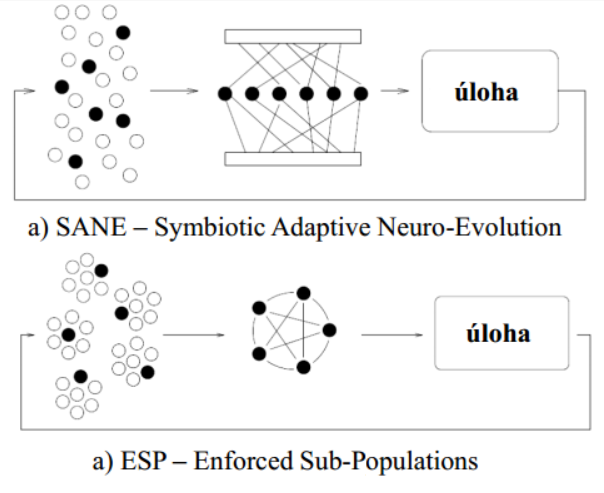
\includegraphics[width=0.5\textwidth]{img/sane_esp.png}
\end{wrapfigure}
\textbf{SANE} (Symbiotic Adaptive Neuroevolution) je variantou neuroevoluce, kdy je struktura pevně daná: jediná skrytá vrstva, pevný počet skrytých neuronů. Jedinci v evoluci jsou neurony (včetně vstupních a výstupních vah). Při ohodnocování se náhodně vybere pevný počet neuronů z populace, postaví se síť a ta se vyhodnotí. Toto se opakuje tak, aby každý neuron z populace byl vybrán aspoň $10\times$. Fitness neuronu je pak průměrná fitness všech sítí, jichž byl součástí.

\textbf{ESP} (Enforced Sub-Populations) funguje na podobném principu, tj. architektura je opět předem daná s pevně daným počtem neuronů (na rozdíl od SANE může být i rekurentní). Rozdíl je v tom, že pro každý z těchto \uv{slotů} se vyvíjejí neurony zvlášť, v oddělených subpopulacích. Takto navržená evoluce podporuje diverzitu (dobrá síť potřebuje různé druhy neuronů), potlačuje redundanci (neurony se vyvíjí pro kompatibilní role) a implicitně rozděluje prohledávaný prostor na podúlohy.


\subsubsection{NEAT (Neuroevolution of Augmenting Topologies)}
Základními charakteristikami algoritmu NEAT jsou: 
\begin{enumerate}
	\leftskip 20pt
	\setlength{\itemsep}{0pt}
	\item evoluce topologie společně s vahami
	\item smysluplné křížení pomocí historických značek
	\item ochrana inovací pomocí druhů
\end{enumerate}
Evoluce topologie zahrnuje přidání/odebrání synapse, přidání/odebrání vrcholu. Typicky se začíná od menší sítě, která postupně roste.

Každý neuron a každý synaptický spoj dostanou při svém vzniku svou \textit{historickou značku} (nebo \uv{rodné číslo}). Tato značka se dědí, takže i u různých potomků lze poznat, zda neurony/spoje mají stejný evoluční původ. Při křížení dvou jedinců se potom postupuje takto: pokud se uzel (neuron či spoj) vyskytuje pouze v jednom rodiči, je automaticky zkopírován; pokud se vyskytuje v obou, je náhodně vybrán jeden z nich.
\begin{figure}[H]
	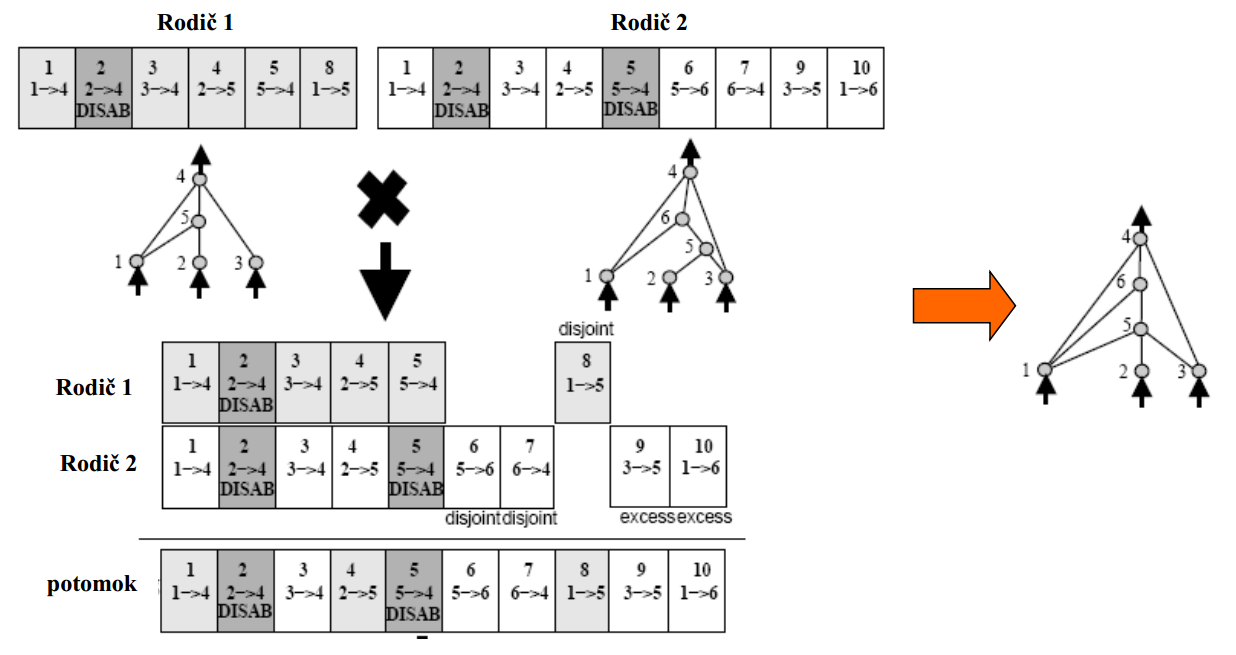
\includegraphics[width=\textwidth]{img/neat.png}
\end{figure}

Když během evoluce vznikne jedinec, který se výrazně liší od ostatních (na to musí být definovaná nějaká metrika), založí se nový \textbf{druh}. Ten je několik generací chráněný -- jedinci nového druhu soutěží pouze mezi sebou.

%TODO hyperneat

\subsection{Řešení kombinatorických úloh}
EA jsou velmi vhodné pro řešení NP-těžkých úloh. Rozebereme několik příkladů:

\subsubsection{Batoh (0-1 knapsack problem)}
\textit{Problém:} máme batoh o kapacitě $CMAX$, množinu $n$ věcí, z nichž každá má cenu $v(i)$ a objem $c(i)$. Úkolem je naplnit batoh tak, abychom maximalizovali sumu cen obsažených věcí a současně nepřekročili kapacitu batohu.

\textbf{Kódování:} Binární jedinci délky $n$, přímočará bitová mapa. Např. 0110010 znamená, že bereme věci s indexy 2,3 a 6. Pozor, jedinci nemusí splňovat podmínku o $CMAX$.

\textbf{Operátory:} Lze použít přímočaré křížení, mutaci a klasickou selekci.

\textbf{Fitness:} Bude mít 2 členy: 
$$\max\limits_{B \subset \{1..n\}} \sum\limits_{i \in B} v(i) \text{\ \ a současně\ \ } \min\limits_{B \subset \{1..n\}} CMAX - \sum\limits_{i \in B} c(i)$$

Problém s víceúčelovou optimalizací lze řešit různě:
\begin{itemize}
	\leftskip 20pt
	\setlength{\itemsep}{0pt}
	\item Oba členy fitness zvážit a sečíst
	\item Použít jeden z obecných EA pro víceúčelové funkce
	\item Anebo chytře změnit zakódování:
	\begin{itemize}	
		\setlength{\itemsep}{0pt}
		\leftskip 20pt
		\item 1 znamená: DEJ věc do batohu POKUD se nepřeplní
		\item takto dosáhneme i toho, že všechny řetězce jsou přípustná řešení
	\end{itemize}
\end{itemize}

\subsubsection{Problém obchodního cestujícího (TSP -- travelling salesman problem)}
\textit{Problém:} Máme $n$ měst, mezi nimi existují cesty definované délky (úplný graf, ohodnocené hrany). Cílem je navštívit všechna města s co nejmenšími náklady -- tj. najít co nejkratší hamiltonovskou kružnici.

\textbf{Fitness:} Délka cesty.

Existuje několik možných reprezentací a na nich závislých genetických operátorů:
\begin{description}
	\leftskip 40pt
	\setlength{\itemsep}{0pt}
	\item[reprezentace sousednosti:] Cesta je seznam měst, město $j$ je na pozici $i$, vede-li cesta z $i$ do $j$. Např. (248397156) odpovídá cestě 1-2-4-3-8-5-9-6-7. Některé seznamy negenerují přípustnou cestu. Klasické křížení nefunguje. Schémata fungují, např (*3*\dots) značí všechny cesty s hranou 2-3.
	\item[reprezentace bufferem] Máme buffer vrcholů, třeba uspořádaný. Reprezentace představuje pořadí města v bufferu, města se z bufferu postupně mažou. Např. buffer (123456789) a reprezentace (112141311) kóduje cestu 1-2-4-3-8-5-9-6-7. V této reprezentaci lze použít jednobodové křížení.
	\item[reprezentace permutací] Nejvíce přímočaré: řetězec (517894623) kóduje cestu 5-1-7-8-9-4-6-2-3. Klasické křížení nefunguje, byly navrženy speciální operátory (dobrý přehled viz \footnote{http://www.rubicite.com/Tutorials/GeneticAlgorithms/CrossoverOperators/PMXCrossoverOperator.aspx}):
	\begin{description}
		\leftskip 30pt
		\setlength{\itemsep}{0pt}
		\item[PMX (partially mapped crossover] Náhodně vybereme podřetězec z rodiče 1, ten zkopírujeme do nového jedince. Pak se podíváme na tytéž pozice v rodiči 2. Pro každou hodnotu, která se ještě nevyskytuje v budovaném potomkovi, budeme hledat vhodné umístění: nechť chceme umístit hodnotu $h$, která se nachází v rodiči 2 na pozici $i$. Vezmeme hodnotu $h_2$ na téže pozici $i$, ale v rodiči 1. Pak se podíváme, kde se $h_2$ nachází v rodiči 2 -- označme tuto pozici jako $i_2$. Je-li to mimo zkopírovanou oblast, pak jsme našli vhodné umístění a zkopírujeme původní hodnotu $h$ do nového potomka na $i_2$. Je-li $i_2$ uvnitř kopírovaného intervalu, pak pokračujeme v hledání -- do $h_2$ dosadíme hodnotu na $i_2$ v rodiči 1. Viz obr. \ref{pmx}.
		\begin{figure}[H]
			\centering			
			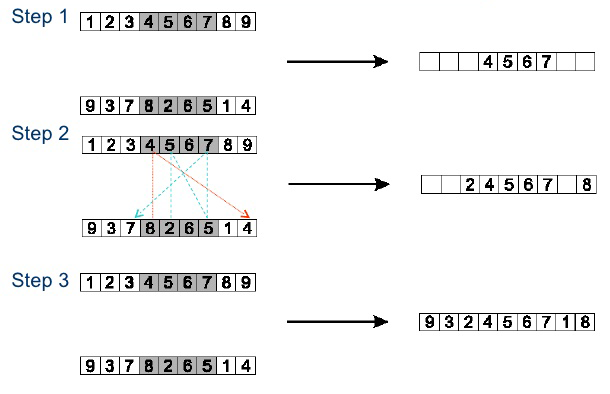
\includegraphics[width=0.6\textwidth]{img/pmx.png}
			\caption{Partially mapped crossover (PMX)}
			\label{pmx}
			
		\end{figure}
		\item[OX (order crossover)] Nejrychlejší křížení. Stejně jako v PMX nejprve vezmeme náhodný podinterval rodiče 1 a beze změny jej zkopírujeme do potomka. Poté vezmeme nepoužité hodnoty z rodiče 2 a počínaje pravým koncem zkopírovaného intervalu je dokopírujeme do potomka.
		
		\begin{figure}[H]
			\centering			
			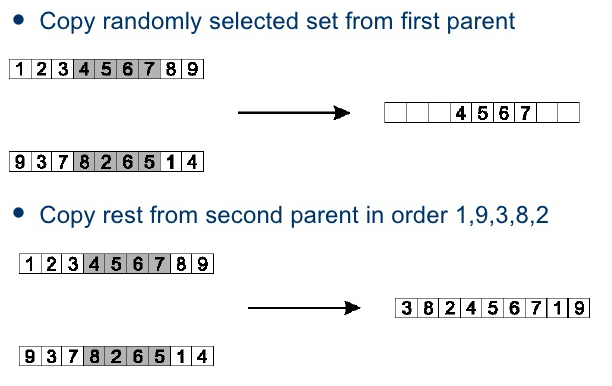
\includegraphics[width=0.6\textwidth]{img/ox.png}
			\caption{Order crossover (OX)}
			\label{pmx}
			
		\end{figure}
		\item[CX (cyclic crossover)] Nejprve jsou identifikovány \uv{cykly} mezi dvěma rodiči: začneme první hodnotou v prvním rodiči, podíváme se na hodnotu na tomtéž indexu v rodiči 2, tuto hodnotu najdeme v rodiči 1, podíváme se na hodnotu na témže indexu v rodiči 2 atd. dokud neuzavřeme cyklus. Takto najdeme všechny cykly. Nového jedince pak vytvoříme kopírováním hodnot po cyklech: hodnoty z prvního cyklu zkopírujeme z prvního rodiče, hodnoty z druhého cyklu z druhého rodiče, hodnoty z třetího cyklu opět z prvního rodiče atd.
		
		\begin{figure}[H]
			\centering			
			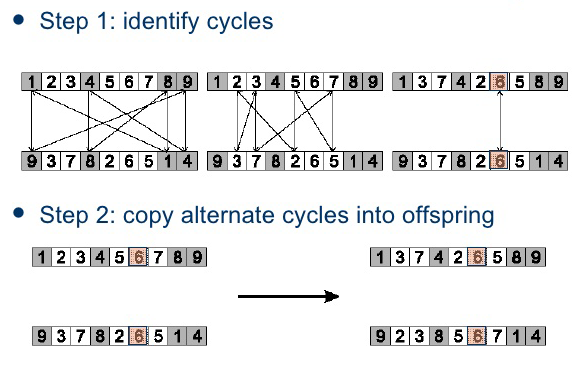
\includegraphics[width=0.6\textwidth]{img/cx.png}
			\caption{Cyclic crossover (CX)}
			\label{cx}
			
		\end{figure}
		
		\item[ER (edge recombination)] Pro každé město si udělám seznam hran, které do/z něj vedou a jsou použity v některém z rodičů. Pak začnu náhodným městem a postupně napojuji další, přičemž vždy ze sousedů vybírám město s nejméně hranami (v případě shody náhodně). Může se stát, že nelze hranu vybrat, ale to se v praxi stává zřídka.
		\item[ER2] Vylepšení: označím si hrany, které jsou dvakrát (tj. v obou rodičích) a při výběru jim dávám přednost. To zachovává ještě více hran z obou rodičů.
		\begin{figure}[H]
			\centering			
			\smallskip
			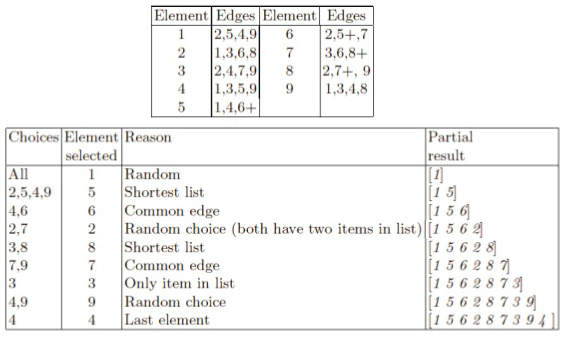
\includegraphics[width=0.6\textwidth]{img/er.png}
			\caption{Edge recombination 2 (ER2): příklad pro rodiče (123456789) a (937826514)}
			\label{pmx}
			
		\end{figure}
		
	\end{description}
\end{description}



Mutace jsou obecně jednodušší (pro všechny reprezentace), používá se:
\begin{itemize}
	\leftskip 20pt
	\setlength{\itemsep}{0pt}
	\item inverze podcesty
	\item posun podcesty
	\item záměna 2 měst
	\item záměna podcest
	\item složitější heuristiky: např. \textbf{2-OPT}. Tento \uv{chytrý operátor} funguje tak, že se vyberou dvě hrany, ty se odeberou a nahradí jinými dvěma hranami (je jen jedna možnost). Nakonec se vybere kratší z obou vzniklých cest. Vlastně se jedná o mutaci, která vezme část cesty a tu vloží do jedince v opačném pořadí. 2-OPT se navíc ještě podívá, jestli je výsledek kratší a přijme ho jen pokud je.
	
	2-OPT se přirozeně dá zobecnit na \textbf{$k$-OPT}, odstraní se $k$ hran a vzniklé fragmenty se pospojují tak, aby výsledná cesta byla co možná nejkratší.
\end{itemize}

Úspěšnost evoluce závisí také na inicializaci. Nejpoužívanější jsou dvě varianty:
\begin{description}
	\leftskip 40pt
	\setlength{\itemsep}{0pt}
	\item[nejbližší sousedi] Začni s náhodným městem, postupně vybírej jako další to nejbližší z dosud nevybraných.
	\item[vkládání hran] Budujeme cestu T, na začátku náhodná hrana. K cestě T vyber nejbližší město c mimo T. Najdi hranu k-j v T tak, že minimalizuje rozdíl mezi k-c-j a k-j. Vyhoď k-j, vlož k-c-j do T.
\end{description}

\subsection{Vícekriteriální optimalizace (MOEA -- Multi-objective EA)}
Velmi často potřebujeme optimalizovat více funkcí současně, tj. místo jedné fitness jich máme celý vektor $\overline{f} = (f_1, f_2, \dots f_n)$. Ty si často odporují, nelze tedy najít řešení optimální pro všechny zároveň.

\begin{wrapfigure}{r}{0.45\textwidth}
	\centering
	
	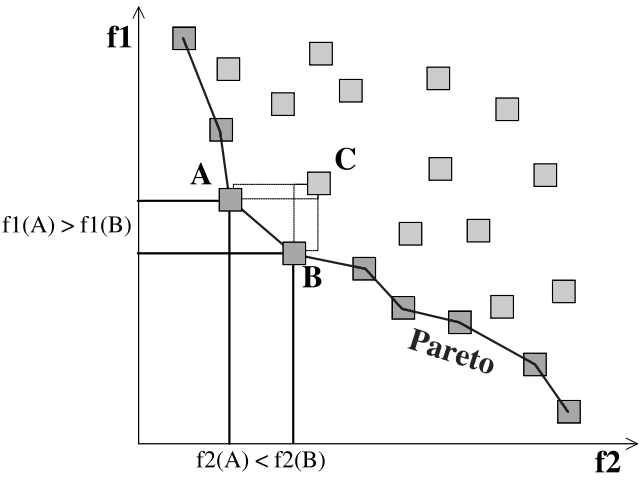
\includegraphics[width=0.4\textwidth]{img/pareto.png}
\end{wrapfigure}

Řekneme, že řešení $x$ \textbf{slabě dominuje} řešení $y$, jestliže $x$ je ve všech kritériích aspoň tak dobré jako $y$, tj. $f_i(x) \leq f_i(y)\quad \forall i \in \{1,\dots,n\}$. 

Řekneme, že $x$ \textbf{dominuje} $y$, když jej slabě dominuje a navíc je aspoň v jedno kritériu lepší, tj. $\exists j: f_j(x) < f_j(y)$. 

Řešení $x$ a $y$ jsou \textbf{nesrovnatelná}, jestliže $x$ nedominuje $y$ a $y$ nedominuje $x$.

\textbf{Pareto-optimální řešení} (Paretova fronta, Pareto-optimální fronta) je množina jedinců, kteří nejsou dominováni žádným jiným jedincem. Je často nekonečná, hledáme konečnou aproximaci.

V případě MOEA není jeden nejlepší jedinec v populaci, používá se celá populace a považuje se za aktuální aproximaci Pareto-optimální množiny řešení. 

\subsubsection{Algoritmy}
Hlavní rozdíl mezi jednokriteriálními a vícekriteriálními algoritmy je v selekci (operátory mohou klidně zůstat stejné). S čímž samozřejmě souvisí způsob, jakým se počítá fitness. Celkově je potřeba zajistit konvergenci k Pareto optimální frontě a zároveň zajistit i dobré pokrytí této fronty.
\begin{description}
	\leftskip 40pt
	\setlength{\itemsep}{0pt}
	\item[Agregace fitness] Nejjednodušší přístup. Definujeme agregovanou fitness $f$ jako váženou sumu všech $f_i$ a problém řešíme jako klasickou jednokriteriální optimalizaci. Problémem je nastavení vah u jednotlivých $f_i$.
	\item[VEGA (Vector Evaluated GA)] Populaci $N$ jedinců utřídím podle každé z $n$ fitness funkcí, poté pro každé $i$ vyberu $\frac{N}{n}$ nejlepších jedinců dle $f_i$. Na ty poté aplikuji křížení, mutaci a provedu selekci do další generace. 
	
	Nevýhodou tohoto přístupu je obtížné udržování diverzity populace a často dochází ke konvergenci k extrémům jednotlivých $f_i$.
	\item[NSGA (Non-dominated sorting GA)] Fitness se počítá pomocí dominance, diverzitu populace zaručuje \textbf{niching}.
	
	Populace $P$ je rozdělena na postupně konstruované fronty $F_1$, $F_2$, \dots, a to takto: 
	\begin{itemize}
		\leftskip 40pt
		\setlength{\itemsep}{0pt}
		\item $F_1$ je množina všech nedominovaných jedinců z $P$
		\item $F_2$ je množina všech nedominovaných jedinců z $P-F_1$
		\item $F_3$ je množina všech nedominovaných jedinců z $P - (F_1 \cup F_2)$
		\item \dots
	\end{itemize}
	
	Pro každého jedince $i$ ve frontě $F_k$ se spočte jeho \textit{niching faktor} jako
	$$sh(i) = \sum_{j \in F_k} sh(i,j)$$
	kde 
	$$
	sh(i,j) = 
	\begin{cases}
		1 - \left(\frac{d(i,j)}{dshare}\right)^2 	& \quad \text{pro $d(i,j) < dshare$} \\
		0 											& \quad \text{jinak}\\
	\end{cases}
	$$
	kde $d(i,j)$ je vzdálenost $i$ a $j$, $dshare$ je předem daný parametr. Niching faktor tedy vyjadřuje, jak blízko jsou další jedinci v populaci. Čím blíže 0, tím osamocenější jedinec je, naopak hodnota blízká 1 znamená mnoho blízkých sousedů.
	
	Jedinci z $F_1$ dostanou nějakou \uv{dummy fitness} dělenou jejich niching faktorem. Jedinci z $F_2$ dostanou jinou dummy fitness, která je menší než fitness nejhoršího jedince z $F_1$ a opět se dělí jejich niching faktorem; atd.
	
	\item[NSGA II] Odstraňuje nutnost určení $dshare$ -- nahrazuje ji \textbf{crowding distance}, což je součet přes všechna kritéria, vzdálenosti nejbližšího horšího (v daném kritériu) a nejbližšího lepšího jedince. Fitness se pak ve skutečnosti nepočítá, namísto toho se v turnajové selekci porovnávají jedinci nejprve podle čísla fronty (menší je lepší), v případě remízy podle crowding distance (větší je lepší -- jedinci jsou v řídce osídlené oblasti a tedy lépe přispívají k pokrytí fronty).
	
	Dále zavádí elitismus: stará a nová generace jsou spojeny, utříděny a z nich se pak vybírá lepší část do další populace. Postupně se kopírují fronty (od nejlepší) dokud se vejdou do populace, z fronty, která se již nevejde celá, se vybírá podle turnajové metody popsané výše.
	
\end{description}

\subsubsection{Porovnání algoritmů}
Pro porovnání kvality řešení dvou různých algoritmů je třeba vyhodnotit, která z výsledných populací lépe aproximuje Pareto optimální množinu. 
\begin{description}
	\leftskip 40pt
	\setlength{\itemsep}{0pt}
	\item[IGD (Inverted Generational Distance)] IGD měří průměrnou vzdálenost každého řeše\-ní na \textit{skutečné} Pareto optimální frontě k nejbližšímu řešení ve výsledné množině. Díky tomu indikátor vyjadřuje jak blízkost řešení k Pareto-optimální frontě (convergence), tak to, jestli jsou řešení po frontě rozmístěna rovnoměrně (spread). Menší hodnoty tohoto indikátoru jsou lepší. 
	\begin{figure}[H]
		\centering
		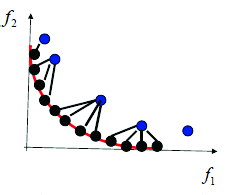
\includegraphics[width=0.4\textwidth]{img/igd.png}
	\end{figure}
	
	\item[Hyperobjem (HV -- hypervolume)] Hyperobjem vyjadřuje objem prostoru dominovaného danou množinou (a omezeného zvoleným referenčním bodem). V případě, že máme jen dvě funkce, které obě najednou minimalizujeme, tak se jedná o plochu \uv{nad} body, které jsou obrazy jedinců v populaci. Plocha je shora omezena referenčním bodem (jinak by byla nekonečná). Tento indikátor opět spojuje jak konvergenci, tak pokrytí Pareto-optimální fronty. Větší hodnoty tohoto indikátoru jsou lepší. Někdy se také jako indikátor používá rozdíl hyperobjemu \textit{skutečné} Pareto optimální fronty a aproximace nalezené algoritmem. Potom jsou samozřejmě lepší menší hodnoty.
	\begin{figure}[H]
		\centering
		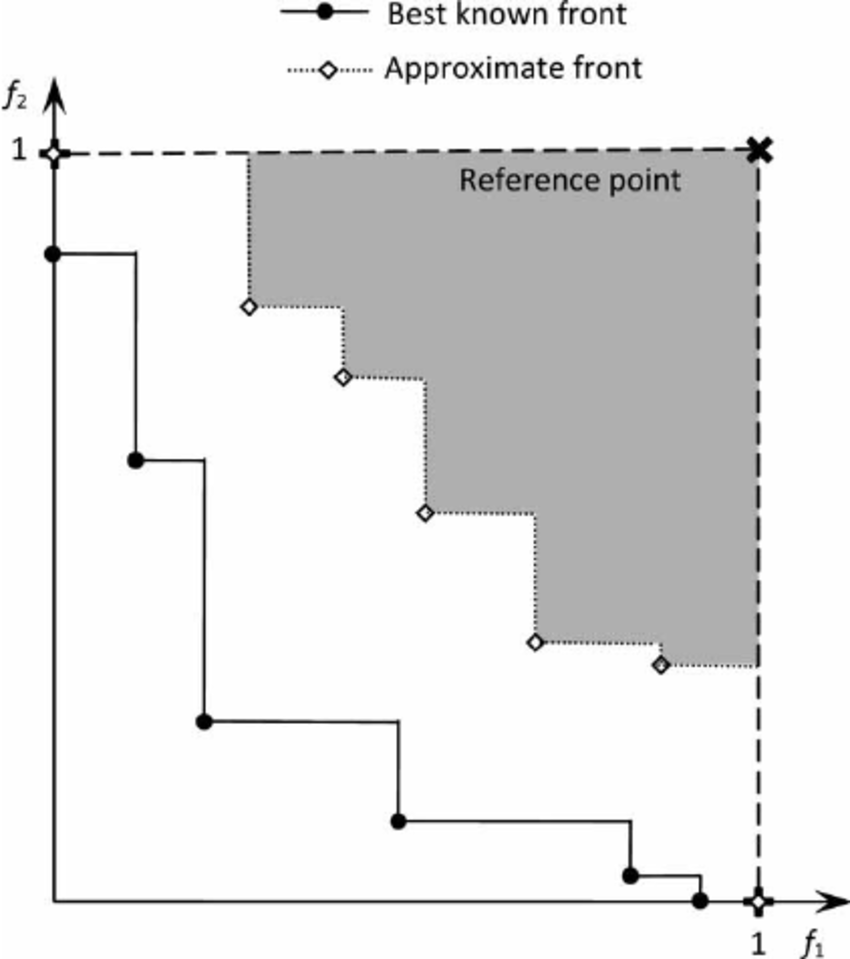
\includegraphics[width=0.35\textwidth]{img/hypervolume.png}
	\end{figure}
	
\end{description}


\part{Strojové učení}
\chapter{Strojové učení a jeho aplikace}
\section{Strojové učení; prohledávání prostoru verzí, učení s učitelem a bez učitele, pravděpodobnostní přístupy, teoretické aspekty strojového učení.}
\section{Evoluční algoritmy; základní pojmy a teoretické poznatky, hypotéza o stavebních blocích, koevoluce, aplikace evolučních algoritmů.}
\section{Strojové učení v počítačové lingvistice a algoritmy pro statistický parsing.}
\section{Pravděpodobnostní algoritmy pro analýzu biologických sekvencí; hledávání motivů v DNA, strategie pro detekci genů a predikci struktury proteinů.}


\chapter{Neuronové sítě}
\section{Neurofyziologické minimum.}
Neuronové sítě jsou výpočetní model inspirovaný lidským mozkem a jeho fungováním, proto rozebereme základní biologické poznatky.

\subsection{Mozek}

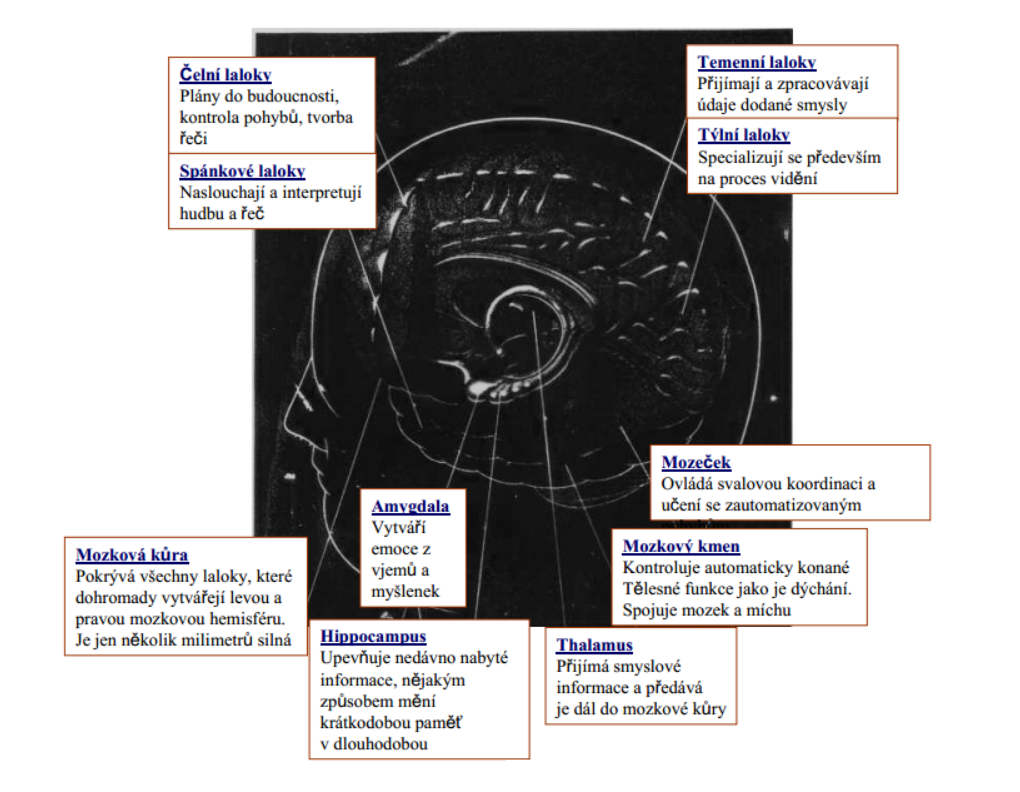
\includegraphics[width=\textwidth]{img/mozek.png}

\subsection{Neuron}
Biologický neuron se skládá z \textbf{těla (somatu)}, \textbf{dendritů} a \textbf{axonu}. Jednotlivé neurony jsou spojeny prostřednictvím \textbf{synapsí}.
\begin{description}
	\leftskip 40pt
	\setlength{\itemsep}{0pt}
	\item[tělo (soma)] Obsahuje organely neuronu včetně jádra (nukleus). Na základě signálů z dendritů může dojít k \textbf{excitaci}.
	\item[dendrity] \uv{Antény} neuronu, místa vstupu signálů z ostatních neuronů (přijímací strana synapse). Místa synapsí jsou pokryta speciální membránou plnou tzv. \textit{receptorů}, které detekují neurotransmittery v synaptické mezeře (\textit{synaptic cleft}). Délka cca 2-3\,mm.
	\item[axon] Jediný výstup neuronu, který však bývá bohatě (typicky pravoúhle) rozvětvený. Přenáší signál k synapsím a dále do ostatních napojených neuronů. Délka může být i přes 1\,m.
	\item[synapse] Místo kontaktu z jiným neuronem. Dochází původně elektrický signál přivedený axonem se zde mění na chemický, který překlene mezeru (\textit{synaptic cleft}) mezi presynaptickou a postsynaptickou plochou (z axonu jednoho neuronu do dendritu jiného neuronu). Na 1 neuron připadá až $10^6$ spojů s jinými neurony.
\end{description}

Kromě neuronů se v mozku nachází ještě \textit{glie}, které mají především podpůrnou funkci. Prvním typem jsou \textbf{astrocyty}, které vyplňují prostor mezi neurony a obalují místa synapsí, čímž brání šíření neurotransmitterů mimo \textit{synaptic cleft}. Druhým typem jsou \textbf{myelinating glia}, které obalují axony (celý obal se nazývá \textit{myelin}). Obálka není zcela souvislá, v pravidelných intervalech je membrána axonu exponována (tzv. \textit{node of Ranvier}).

\begin{figure}[H]
	\centering
	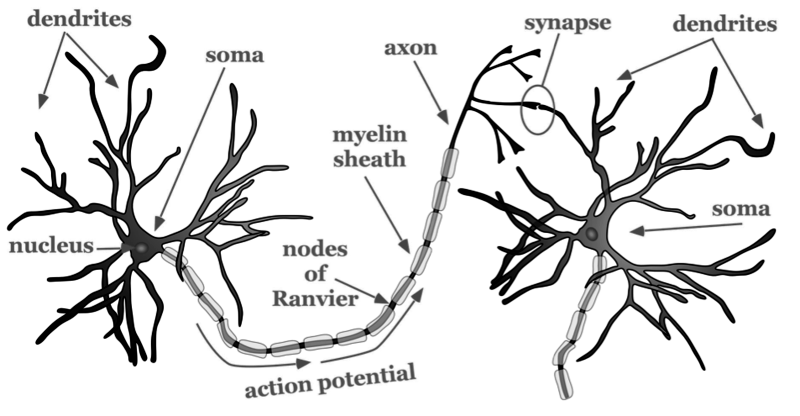
\includegraphics[width=0.7\textwidth]{img/neuron.png}
\end{figure}


\subsection{Přenos signálu}
Obal neuronu tvoří \textit{membrána}, která se skládá ze dvou vrstev molekul \textbf{fosfolipidů}. V membráně jsou umístěny \textbf{iontové pumpy} a \textbf{kanály}. Iontové kanály volně propouští ionty daného typu, iontové pumpy je přenáší aktivně a spotřebovávají přitom energii (ve formě ATP). Každý kanál či pumpa jsou selektivní vůči jednomu typu iontů: především K$^+$, Na$^+$ a Cl$^-$.

\subsubsection{Klidový potenciál}
Pomocí pump je udržována neustálá \textbf{polarizace membrány}. Vně je kladný potenciál, uvnitř záporný (rozdíl se pohybuje kolem -70\,mV). Nejvíce prominentní jsou sodíkovo-draslíkové pumpy, které pumpují K$^+$ dovnitř a současně Na$^+$ ven. Draslíkové kanály jsou otevřené, takže nepoměr koncentrace draslíkových iontů vně a uvnitř se může vyrovnávat. Sodíkové kanály jsou ovšem uzavřené, takže sodík zůstává více koncentrovaný vně. To vede k zápornému potenciálu uvnitř neuronu.

\begin{figure}[H]
	\centering
	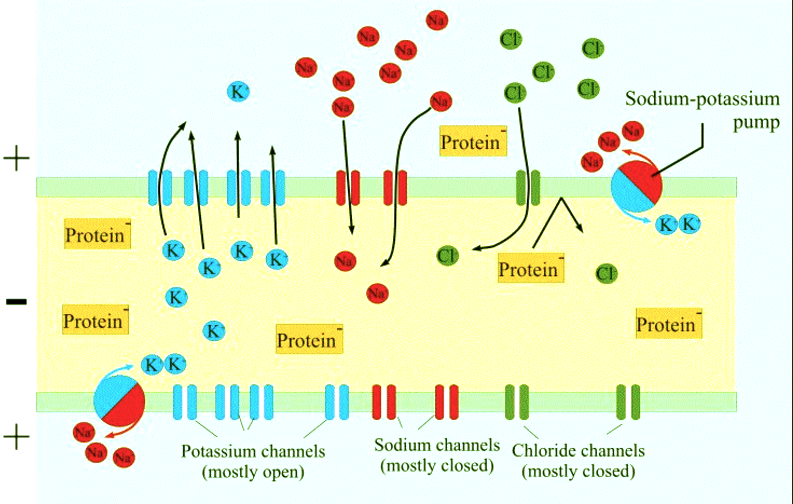
\includegraphics[width=0.7\textwidth]{img/resting_potential.png}
\end{figure}


\subsubsection{Akční potenciál}
Některé Na$^+$ a K$^+$ kanály jsou \textit{voltage-gated}, tj. při dosažení jisté úrovně napětí (-55\,mV) dochází k jejich automatickému uzavření/otevření. Tím je umožněno generování akčního potenciálu. Přílivem Na$^+$ (například z jiného neuronu, vybuzením receptorů v dendritech) dochází k depolarizaci neuronu. Dosáhne-li depolarizace kritické úrovně (\textit{threshold}), dojde k uzavření K$^+$ kanálů a otevření Na$^+$ kanálů a rapidnímu přílivu Na$^+$ dovnitř neuronu, neboť v něm je stále negativní potenciál. Tzv. \textit{rising phase}. Příliv je natolik veliký, že dojde k tzv. \textit{overshoot}, kdy je vnitřek neuronu nabit kladně na cca 40\,mV. V tuto chvíli dochází k uzavření Na$^+$ kanálů a otevření K$^+$ kanálů a potenciál se opět začíná snižovat - tzv. \textit{falling phase}. Jelikož je otevřeno více K$^+$ kanálů než obvykle (klasické + voltage-gated), dochází k tzv. \textit{undershoot}, tj. hyperpolarizaci neuronu. Po zavření voltage-gated kanálů se napětí opět ustálí na klidovém potenciálu.
\begin{figure}[H]
	\centering
	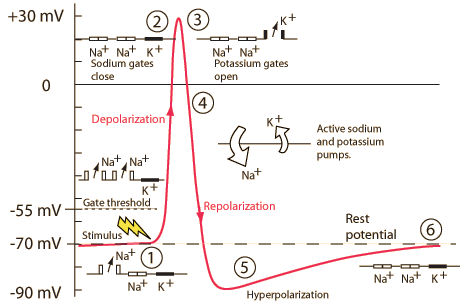
\includegraphics[width=0.7\textwidth]{img/action_potential.png}
\end{figure}

\subsection{Paměť}
\begin{description}
	\leftskip 40pt
	\setlength{\itemsep}{0pt}
	\item[Krátkodobý paměťový mechanismus] Založen na cyklickém oběhu vzruchů v neuronových sítích. Proběhne-li tato cirkulace cca 300-krát, začne docházet k fixaci informace ve střednědobé paměti – to trvá cca 30 s.
	\item[Střednědobý paměťový mechanismus] Založen na změnách \uv{vah neuronů}. Změna váhových koeficientů v synapsi je vyvolána mnohonásobným působením téhož signálu na příslušných synaptických přechodech. Ve spánku přecházejí některé z takto uchovaných informací do dlouhodobých pamětí. Informace se uchovává několik hodin a případně i dnů.
	\item[Dlouhodobý paměťový mechanismus] Spočívá v kopírování informací ze střednědobé paměti do bílkovin, které jsou uvnitř neuronů – hlavně v jejich jádrech. Některé takto uchovávané informace zůstanou v organismu celý život.
\end{description}


\section{Modely pro učení s učitelem, algoritmus zpětného šíření, strategie pro urychlení učení, regularizační techniky a generalizace.}

\subsection{Modely pro učení s učitelem}
\subsubsection{Formální neuron}
\textbf{Formální neuron} s vahami $(w_1, w_2, \dots w_n) \in \R^n$, prahem $\theta \in \R$ a přenosovou funkcí $f : \R^{n+1} \times \R^n \rightarrow \R$ počítá pro libovolný vstup $\vec{x} \in \R^n$ svůj výstup $y$ jako hodnotu přenosové funkce $f$ v $\vec{x}$, $f[\vec{w}, \theta](\vec{z})$. Mezi nejznámější \textbf{přenosové funkce} (také \textbf{aktivační funkce}) patří \textit{skoková} (unit step), \textit{sigmoidální} nebo \textit{hyperbolická tangentoida}. \textbf{Potenciál neuronu} je vážená suma jeho vstupů: $\xi = \sum\limits_{i=1}^n x_i w_i + \theta$. Právě tento potenciál je vstupem přenosové funkce (na přehledu níže je potenciál neuronu označen písmenem $z$).

\begin{figure}[H]
	\centering
	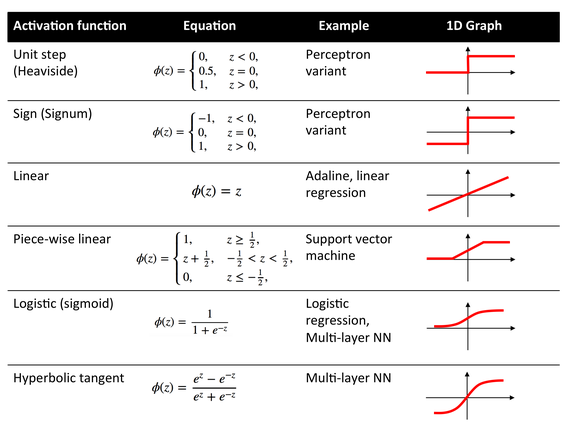
\includegraphics[scale=0.7]{img/activation_functions.png}
\end{figure}

\subsubsection{Perceptron}
\textbf{(Jednoduchý) perceptron} je výpočetní jednotka sestávající z jediného neuronu se skokovou přenosovou funkcí, tj.
\[
y = f[\vec{w},\theta](\vec{x}) = 
\begin{cases}
1 	& \quad \sum\limits_{i=1}^n w_i x_i \geq \theta \quad \text{tedy pokud} \quad \vec{w}\cdot\vec{x} \geq \theta\\
0 	& \quad \text{jinak}\\
\end{cases}
\]
Často se uvažuje tzv. \textbf{rozšířený váhový a vstupní vektor}, kde je navíc umělý vstup s konstantní hodnotou 1 a vahou $-\theta$, tj. $\overrightarrow{w_{ext}} = (w_1, w_2, \dots, w_n, -\theta)$, $\overrightarrow{x_{ext}} = (x_1, x_2, \dots, x_n, 1)$. Potom lze práh neuronu považovat za váhu speciálního vstupu a přenosovou funkci počítat jako 

\[
y = f[\vec{w},\theta](\vec{x}) = 
\begin{cases}
1 	& \quad \overrightarrow{w_{ext}}\cdot\overrightarrow{x_{ext}} \geq 0\\
0 	& \quad \text{jinak}\\
\end{cases}
\]

Jednoduchý perceptron ve skutečnosti realizuje \textbf{dělící nadrovinu}, jejíž poloha je dána váhovým vektorem: je to množina všech bodů $\vec{x} \in \R$, pro něž $\vec{w}\cdot\vec{x} = 0$. Ve dvourozměrném případě odpovídá perceptron dělicí přímce. Všechny body na jedné straně přímky jsou perceptronem klasifikovány jako 1, všechny body na druhé straně jako 0. Formálně mluvíme o \textit{pozitivním a negativním podprostoru}: \textbf{otevřený (uzavřený) pozitivní podprostor} určený váhovým vektorem $\vec{w}$ je množina všech bodů $\vec{x} \in \R$, pro něž $\vec{w}\cdot\vec{x} > 0$ ($\vec{w}\cdot\vec{x} \geq 0$). \textbf{Negativní podprostor} je definován analogicky.

Abychom mohli formulovat typy úloh, které perceptron umí řešit, budeme také potřebovat následující definici:

Dvě množiny $A$ a $B$ se nazývají \textbf{lineárně separabilní} v $n$-rozměrném prostoru, pokud existuje $n+1$ reálných čísel $w_1, w_2, \dots w_n, \theta$ takových, že každý bod $\vec{x} = (x_1, x_2, \dots, x_n) \in A$ splňuje $\sum\limits_{i=1}^n w_i x_i \geq \theta$ a každý bod $\vec{x} = (x_1, x_2, \dots, x_n) \in B$ splňuje $\sum\limits_{i=1}^n w_i x_i < \theta$. Pokud dokonce v obou případech platí ostrá nerovnost, mluvíme o \textbf{absolutní lineární separabilitě}. 

Lze dokázat, že pokud jsou dvě množiny separabilní, jsou i absolutně separabilní (idea důkazu: posun přímky o $\sfrac{\varepsilon}{2}$).

Nalezení vhodné dělicí nadroviny pro zadané body je ekvivalentní nalezení vhodného vektoru $\vec{w}$. To probíhá pomocí \textbf{perceptronového učení}:
\begin{enumerate}
	\leftskip 40pt
	\setlength{\itemsep}{0pt}
	\item inicializace vah náhodnými hodnotami $w_i(0)$
	\item předložení trénovacího vzoru, tj. $\vec{x} = (x_1, x_2,\dots,x_n)$ a očekávaného výstupu $d(t)$
	\item výpočet skutečného výstupu jako $y(t) = sgn(\vec{w}\cdot\vec{x})$
	\item adaptace vah:
	\begin{align*}
		w_i(t+1)& = w_i(t)			& \text{výstup je správný}\\
		w_i(t+1)& = w_i(t) + x_i	& \text{výstup je 0 a měl být 1}\\
		w_i(t+1)& = w_i(t) - x_i	& \text{výstup je 1 a měl být 0}
	\end{align*}
	\item pokud $t$ nedosáhl požadované hodnoty, přejdi ke kroku 2
\end{enumerate}

Základním principem je natáčení vektoru $\vec{w}$ (který je kolmý na dělicí nadrovinu) ve směru kladných vzorků. Je-li výstupv kroku 3 kladný, svírají $\vec{w}$ a $\vec{x}$ úhel menší než 90\,°, je-li záporný, je úhel větší než 90\,°. 

Pro nastavení počátečních vah může být použita jednoduchá heuristika: vezmi průměr kladných vstupů mínus průměr záporných vstupů.

Další heuristikou je použít parametr učení $\eta \in (0,1)$, který ovlivňuje plasticitu modelu. Váhy se pak aktualizují podle $w_i(t+1) = w_i(t) + \eta\cdot x_i$, resp. $w_i(t+1) = w_i(t) - \eta\cdot x_i$.

\medskip\noindent\textbf{Věta (konvergence perceptronového algoritmu učení):} \textit{Nechť P a N jsou konečné a lineárně separabilní množiny. Potom provede perceptronový algoritmus učení konečný počet aktualizací váhového vektoru $\vec{w}$.}

\begin{proof}
Nejprve provedeme 3 zjednodušení:
\begin{enumerate}
	\leftskip 40pt
	\setlength{\itemsep}{0pt}
	\item Sjednotíme $P$ a $N$ jako $P' = P \cup N^-$, kde $N^-$ jsou negované prvky $N$.
	\item Vektory $P'$ normalizujeme.
	\item Váhový vektor bude také normalizovaný. Předpokládané řešení označíme jako $\vec{w^*}$.
\end{enumerate}

Nyní uvážíme situaci v kroku $t$, kdy došlo k aktualizaci váhového vektoru pomocí nějakého $\vec{p_i} \in P'$, tedy $\vec{w_{t+1}} = \vec{w_t} + \vec{p_i}$ (pro přehlednost přesuneme $t$ do dolního indexu). Nyní budeme zkoumat úhel mezi $\vec{w^*}$ a $\vec{w_{t+1}}$, konkrétně výraz:
\begin{equation}
\label{perc_cos}
\cos{\rho} = \frac{\vec{w^*} \cdot \vec{w_{t+1}}}{||\vec{w_{t+1}}||}
\end{equation}

Pro výraz v čitateli víme, že:
$$\vec{w^*}\cdot\vec{w_{t+1}} = \vec{w^*}\cdot(\vec{w_{t}} + \vec{p_i}) = \vec{w^*}\cdot\vec{w_{t}} + \vec{w^*}\cdot\vec{p_i} \geq \vec{w^*}\cdot\vec{w_{t}} + \delta$$ 
kde $\delta = min\{\vec{w^*}\cdot\vec{p}\ |\ \forall\vec{p} \in P'\}$. Protože $\vec{w^*}$ definuje \textit{absolutní} lineární separaci $P$ a $N$, víme, že $\delta > 0$. Indukcí dostáváme
\begin{equation}
	\label{perc_nomin}
	\vec{w^*}\cdot\vec{w_{t+1}} \geq \vec{w^*}\cdot\vec{w_0} + (t+1)\delta
\end{equation}

Pro výraz ve jmenovateli platí
$$||\vec{w_{t+1}}||^2 
= (\vec{w_{t}} + \vec{p_i}) \cdot (\vec{w_{t}} + \vec{p_i}) 
= ||\vec{w_t}||^2 + 2\vec{w_t}\cdot\vec{p_i} + ||\vec{p_i}||^2
$$

Všechny vektory v $P'$ jsou normalizovány, takže poslední člen je roven 1. Navíc $\vec{w_t}\cdot\vec{p_i} \leq 0$ (jinak by nebylo třeba aktualizovat váhový vektor), takže dostáváme
$$
||\vec{w_{t+1}}||^2 \leq ||\vec{w_t}||^2 + ||\vec{p_i}||^2 \leq ||\vec{w_t}||^2 + 1
$$
a indukcí dostaneme
\begin{equation}
\label{perc_denom}
||\vec{w_{t+1}}||^2 \leq ||\vec{w_0}||^2 + (t+1)
\end{equation}

Porovnáním \ref{perc_nomin} a \ref{perc_denom} s původní \ref{perc_cos} dostáváme nerovnici
$$
\cos\rho \geq \frac{\vec{w^*}\cdot\vec{w_0} + (t+1)\delta}{\sqrt{||\vec{w_0}||^2 + (t+1)}}
$$

Pravá strana nerovnice roste proporcionálně k $\sqrt{t}$, a protože $\delta > 0$, mohla by být libovolně velká. Protože ale $\cos\rho \leq 1$, musí existovat horní mez a počet aktualizací váhového vektoru musí být konečný.

\end{proof}

Zmíníme ještě, že popsaný algoritmus není jediný. Existují různé varianty a vylepšení, ve slajdech pí. Mrázové je popsán ještě \textit{přihrádkový algoritmus}.

\subsubsection{Neuronová síť}
\textbf{Neuronová síť} je uspořádaná 6-tice $M=(N,C,I,O,w,t)$, kde:
\begin{itemize}
	\leftskip 40pt
	\setlength{\itemsep}{0pt}
	\item $N$ je konečná neprázdná množina neuronů
	\item $C \subseteq N \times N$ je neprázdná množina orientovaných spojů mezi neurony
	\item $I \subseteq N$ je neprázdná množina vstupních neuronů
	\item $O \subseteq N$ je neprázdná množina výstupních neuronů
	\item $w: C \rightarrow \R$ je váhová funkce
	\item $t: N \rightarrow \R$ je prahová funkce
\end{itemize}

Neurony jsou typicky uspořádány do vrstev, pak mluvíme o \textbf{vrstevnatých sítích}. První vrstva je \textbf{vstupní vrstva} sestávající ze vstupních neuronů, ty nemají v grafu spojů žádné předchůdce a \textbf{jejich výstup je roven jejich vstupu}. Poslední vrstva je \textbf{výstupní vrstva} obsahující výstupní neurony. Zbylé vrstvy jsou \textbf{skryté vrstvy}. 

Typicky uvažujeme sítě s acyklickým grafem spojů, tzv. \textbf{dopředné sítě (angl. feed-forward networks)}. Sítě obsahující cykly nazýváme obecně \textbf{rekurentní sítě}.

\subsection{Algoritmus zpětného šíření (Backpropagation)}
Nejpoužívanější algoritmus učení pro neuronové sítě. Cílem učení je nastavit váhy sítě tak, aby síť správně počítala výstupy pro předkládané vzory. Přitom však není specifikována ani skutečná, ani očekávaná aktivita skrytých neuronů. Jedná se o tzv. \textit{gradientní metodu}, tzn. snaží se minimalizovat nějakou (chybovou) funkci, k čemuž využívá kroky ve směru gradientu funkce v aktuálním bodě.

Pro konečnou množinu trénovacích vzorů $T$ lze celkovou chybu vyjádřit pomocí rozdílu mezi skutečným a
požadovaným výstupem sítě u každého předloženého vzoru. Definujeme tedy \textbf{chybovou funkci} jako
$$E = \frac{1}{2} \sum\limits_{p \in T}\sum\limits_{j\in O}(y_{j,p} - d_{j,p})^2$$
kde $T$ je trénovací množina, $O$ jsou výstupní neurony, $y_{j,p}$ je skutečný výstup neuronu $j$ pro vzor $p$ a $d_{j,p}$ je očekávaná odezva neuronu $j$ na vzor $p$. Používá se kvadratická chyba, aby se zanedbal směr chyby. Zlomek $\sfrac{1}{2}$ je ve vzorci pouze pro pohodlnější počítání při pozdějším derivování. 

Cílem učení je minimalizovat chybu na dané trénovací množině. Úprava vah sítě probíhá iterativně, tj. předloží se vzor, porovná se skutečný a očekávaný výstup, spočte se chyba, adaptují se váhy a pak se pokračuje dalším vzorem. Váhy se upravují od výstupní vrstvy směrem ke vstupní a \textit{proti gradientu chybové funkce}.

Dlužno poznamenat, že síť je po naučení ještě třeba otestovat na nezávislé testovací množině, aby se stanovila její úspěšnost.

\subsubsection{Adaptační pravidla}
V každém kroku aktualizujeme váhy:
$$
w_{ij}(t+1) = w_{ij}(t) + \Delta_E w_{ij}(t)
$$
kde $w_{ij}$ je váha spoje mezi neurony $i$ a $j$; a $\Delta_E w_{ij}(t)$ je přírůstek váhy přispívající k minimalizaci chyby $E$. Ten nalezneme \uv{derivací chyby ve směru této váhy}, kteroužto hodnotu pak odečteme:
$$
\Delta_E w_{ij}(t) 
= -\frac{\partial E}{\partial w_{ij}} 
= -\frac{\partial E}{\partial y_j} \cdot \frac{\partial y_j}{\partial \xi_j} \cdot \frac{\partial \xi_j}{\partial w_{ij}}
$$
Hodnota $y_j$ je skutečný výstup neuronu $j$ a $\xi_j$ je potenciál neuronu $j$, tj. vážená suma jeho vstupů. Tento vzorec ještě dále upravíme, a to zvlášť pro výstupní vrstvu a pro skryté vrstvy. 

\paragraph{Aktualizace synaptických vah pro výstupní vrstvu:}
\begin{align*}
\Delta_E w_{ij}(t) 
&\cong -\frac{\partial E}{\partial y_j} \cdot \frac{\partial y_j}{\partial \xi_j} \cdot \frac{\partial \xi_j}{\partial w_{ij}}\\
&= -\frac{\partial E}{\partial y_j} \cdot \frac{\partial y_j}{\partial \xi_j} \cdot \frac{\partial}{\partial w_{ij}}\sum\limits_{i'} w_{i'j}y_{i'}\\
&\stackrel{(1)}{=} -\frac{\partial E}{\partial y_j} \cdot \frac{\partial y_j}{\partial \xi_j} \cdot y_{i}\\
&\stackrel{(2)}{=} -\frac{\partial E}{\partial y_j} \cdot f'(\xi_j) \cdot y_{i}\\
&\stackrel{(3)}{=} -(y_j - d_j) \cdot f'(\xi_j) \cdot y_{i} = \delta_j \cdot y_{i}\\
\end{align*}

Rovnost (1) platí, neboť v sumě je pouze jediný člen, v němž se vyskytuje \uv{proměnná} $w_ij$, a to $w_{ij}y_i$, který bude po derivaci roven $y_i$. Ostatní členy jsou vůči $w_{ij}$ konstatní a jejich derivace je tedy 0.

Rovnost (2) pracuje pouze s jiným vyjádřením druhého zlomku. Neboť $y_j = f(\xi_j)$ a tedy druhý zlomek je vlastně pouze jednoduchá derivace přenosové funkce.

Rovnost (3) platí triviálně z definice chybové funkce. Ta je suma rozdílů $(y_k - d_k)$, z nichž pouze jediný zůstane po derivaci nenulový. Celkovou derivaci chyby $E$ podle potenciálu $\xi_j$ označíme symbolem $\delta_j$ (bude se nám to hodit později).

\paragraph{Aktualizace synaptických vah pro skryté vrstvy:}
\begin{align*}
\Delta_E w_{ij}(t) 
&\cong -\frac{\partial E}{\partial y_j} \cdot \frac{\partial y_j}{\partial \xi_j} \cdot \frac{\partial \xi_j}{\partial w_{ij}}\\
&\stackrel{(1)}{=} -\frac{\partial E}{\partial y_j} \cdot f'(\xi_j) \cdot y_i\\
&\stackrel{(2)}{=} -\left(\sum\limits_k\frac{\partial E}{\partial\xi_k}\cdot\frac{\partial\xi_k}{\partial y_j} \right) \cdot f'(\xi_j) \cdot y_i \\
&= -\left(\sum\limits_k\frac{\partial E}{\partial\xi_k}\cdot\frac{\partial}{\partial y_j}\sum\limits_{j'}w_{j'k}y_{j'} \right) \cdot f'(\xi_j) \cdot y_i \\
&\stackrel{(3)}{=} -\left(\sum\limits_k\frac{\partial E}{\partial\xi_k}\cdot w_{jk} \right) \cdot f'(\xi_j) \cdot y_i \\
&\stackrel{(4)}{=} -\left(\sum\limits_k \delta_k\cdot w_{jk} \right) \cdot f'(\xi_j) \cdot y_i = \delta_j \cdot y_i\\
\end{align*}

Rovnost (1) plyne stejně, jako v předchozím případě (zestručněno). 

Rovnost (2) platí, neboť $y_j$ již není výstup neuronu ve výstupní vrstvě, který by šlo přímo porovnat s očekávaným výstupem, nýbrž výstup nějakého vniřního neuronu. Budeme tedy iterovat přes všechny neurony $k$, do nichž vede spoj z $j$ (a $y_j$ tedy přispívá do potenciálu $\xi_k$) a tak vyjádříme vliv $y_j$ na celkovou chybu takto nepřímo. 

Rovnost (3) platí analogicky jako rovnost (1) v předchozím případě.

Rovnost (4) využívá označení $\delta_j$ zavedeného v předchozím případě. Jak je vidět, pro úpravu vah vedoucích do vnitřního neuronu $j$ potřebujeme znát $\delta_k$ pro všechny vrcholy $k$, do nichž vede z $j$ hrana. Toto vynucuje počítat směrem od výstupní vrstvy, neboť pro všechny výstupní neurony umíme $\delta_k$ jednoduše spočíst. Pak můžeme spočítat $\delta_k$ (a aktualizace vah) pro předposlední vrstvu, pak pro před-předposlední atd.

Než přejdeme k finálnímu sjednocení vzorců a vyjádření aktualizace vah, vyjádříme si ještě $f'(\xi_j)$. Pracujeme se \textit{sigmoidální přenosovou funkcí}, tj. $f(\xi_j) = \frac{1}{1 + e^{-\lambda\xi_j}}$. Pro tu platí zajímavá a užitečná věc, a to že $f'(\xi_j) = \lambda f(\xi_j)(1 - f(\xi_j))$ neboli $f'(\xi_j) = \lambda y_j(1 - y_j)$.

Nyní tedy umíme vyjádřit přírůstek váhy jako
$$
w_{ij}(t+1) = w_{ij}(t) + \alpha\delta_jy_i
$$
kde
$$
\delta_j =
\begin{dcases*}
(d_j - y_j)\lambda y_j (1-y_j) 	& \quad pro výstupní neuron\\
\left(\sum\limits_k \delta_k\cdot w_{jk} \right) \lambda y_j (1-y_j)  	& \quad pro skrytý neuron\\
\end{dcases*}
$$
Parametr $\alpha \in (0,1)$ nazýváme \textbf{parametrem učení}.

Posledním kouskem skládačky je přidání členu reprezentujícího setrvačnost učení:
$$
w_{ij}(t+1) = w_{ij}(t) + \alpha\delta_jy_i + \alpha_m(w_{ij}(t) - w_{ij}(t-1))
$$
kde $\alpha_m$ nazýváme \textbf{moment učení}. Vyvážení parametrů $\alpha$ a $\alpha_m$ určuje, nakolik se učení řídí gradientem a nakolik setrvačností.

Nyní se pokusíme celý algoritmus zpětného šíření stručně shrnout:

\noindent\fbox{
	\setlength{\fboxsep}{30pt}
	\parbox{\textwidth}{
		Krok 1: Zvolte náhodné hodnoty synaptických vah.\\
		Krok 2: Předložte nový trénovací vzor ve tvaru:
			$$[\ \text{vstup } \vec{x}, \text{požadovaný výstup }\vec{d}\ ]$$
		Krok 3: Vypočtěte skutečný výstup. Aktivita neuronů v každé vrstvě je dána pomocí:
			$$y_j = f(\xi_j) = \frac{1}{1 + e^{-\lambda\xi_j}} , \quad \text{kde } \xi_j = \sum\limits_i{w_{ij}y_i}$$
		Krok 4: Aktualizujte váhy postupně směrem od výstupní vrstvy ke vstupní podle vzorce
			$$
			w_{ij}(t+1) = w_{ij}(t) + \alpha\delta_jy_i + \alpha_m(w_{ij}(t) - w_{ij}(t-1))
			$$
			\hskip 40pt kde
			$$
			\delta_j =
			\begin{dcases*}
				(d_j - y_j)\lambda y_j (1-y_j) 	& \quad pro výstupní neuron\\
				\left(\sum\limits_k \delta_k\cdot w_{jk} \right) \lambda y_j (1-y_j)  	& \quad pro skrytý neuron\\
			\end{dcases*}
			$$
			\hskip 40pt a dále
			\begin{itemize}
				\leftskip 40pt
				\setlength{\itemsep}{0pt}
				\item $w_{ij}(t)$ je váha spoje z neuronu $i$ do neuronu $j$ v čase $t$
				\item $\alpha$ je parametr učení
				\item $\alpha_m$ je moment učení
				\item $\xi_j$ je potenciál neuronu $j$
				\item $\delta_j$ je chyba na neuronu $j$
				\item $k$ je index pro neurony z vrstvy nad neuronem $j$
				\item $\lambda$ je strmost přenosové funkce
			\end{itemize}
		Krok 5: Přejdi ke kroku 2.
			
	}
}

\subsection{Strategie pro urychlení učení}
Popsaný standardní model zpětného učení je poměrně jednoduchý, dává poměrně dobré výsledky, ale má i mnohé nevýhody. V první řadě je docela pomalý. Problém učení neuronových sítí je obecně NP-úplný a výpočetní složitost roste exponenciálně s počtem proměnných. Důležité je taky počáteční nastavení parametrů. 

Existují různé postupy a algoritmy pro urychlení učení. Některé zachovávají pevnou topologii sítě, jiné jsou naopak založeny na použití modulárních sítí, některé algoritmy adaptují jak parametry (váhy, prahy, \dots) i topologii.

\subsubsection{Volba počátečních vah}
Příliš malé počáteční váhy mohou \uv{paralyzovat učení}, tj. propagovaná chyba je příliš malá. Příliš velké váhy naopak vedou k \uv{saturaci} neuronů a rovněž pomalému učení. Oba extrémy mají pak za následek ukončení učení v suboptimálním lokálním extrému. Správná volba počátečních vah může toto riziko výrazně snížit.

\section{Asociativní paměti, Hebbovské učení a hledání suboptimálních řešení, stochastické modely.}
\subsection{Asociativní paměti}
Principem asociativních sítí (a pamětí) je mapování vstupních vektorů $\vec{x}$ na dané výstupní vzory $\vec{y}$, přičemž blízké okolí $\vec{x}$ by se mělo mapovat na týž cílový vzor -- ten se tedy chová jako \uv{araktor}. Asociativní paměti by tedy měly být schopné správně přiřadit vzor i zašuměným vstupům. 

Rozlišujeme 3 základní typy asociativních sítí:
\begin{description}
	\leftskip 40pt
	\setlength{\itemsep}{0pt}
	\item[heteroasociativní sítě] Zobrazují $m$ vstupních vzorů $\vec{x}^1, \vec{x}^2, \dots, \vec{x}^m$ z $n$-rozměrného prostoru na $m$ výstupních vektorů $\vec{y}^1, \vec{y}^2, \dots, \vec{y}^m$ v $k$-rozměrném prostoru tak, že $\vec{x}^i \mapsto \vec{y}^i$. 
	
	Jestliže pro nějaký vektor $\vec{x}$ platí, že $||\vec{x} - \vec{x}^i|| < \varepsilon$, potom $\vec{x} \mapsto \vec{y}^i$ (pro zvolené $\varepsilon > 0$).
	
	\item[autoasociativní sítě] Podmnožina heteroasociativních sítí: každý vzor se zobrazuje 
	sám na sebe, tj. $\vec{y}^i = \vec{x}^i \quad \forall i = 1, \dots, m$. Funkcí těchto sítí je oprava zašuměných vzorů.
	
	\item[sítě pro rozpoznávání vzorů] Speciální typ heteroasociativních sítí, kde je každému vektoru $\vec{x}^i$ přiřazena skalární hodnota $i$, která reprezentuje třídu daného vzoru. Cílem je identifikace třídy daného vstupního vzoru.
\end{description}

\subsubsection{Struktura asociativních pamětí}
Asociativní paměť lze implementovat pomocí jedné vrstvy neuronů (resp. jedné vstupní a jedné výstupní). Síť má $n$ vstupních a $k$ výstupních neuronů. Označíme $w_{ij}$ váhu mezi neurony $i$ a $j$. Pak $\vec{W}$ bude \textbf{matice vah} o rozměrech $n \times k$. Vektor potenciálů výstupních neuronů označíme jako \textbf{excitační vektor} $\vec{e} = \vec{x}\cdot \vec{W}$. V případě identické přenosové funkce na výstupních neuronech pak dostáváme \textit{lineární asociátor} a výstup sítě spočteme jako $\vec{y} = \vec{x} \cdot \vec{W}$.

Nechť $\vec{X}$ je $m \times n$ matice vstupních vzorů a $\vec{Y}$ je $m \times k$ matice výstupních vzorů. Pak lze problém vyjádřit maticově: hledáme $\vec{W}$ tak, aby $\vec{X}\cdot \vec{W} = \vec{Y}$ (v případě autoasociativní paměti $\vec{X}\cdot \vec{W} = \vec{X}$). Pokud je $\vec{X}$ čtvercová a regulární, lze řešení najít jednoduše jako $\vec{W} = \vec{X}^{-1} \cdot \vec{Y}$. Obecně to ale samozřejmě platit nemusí.

\subsubsection{Rekurentní asociativní síť}
Než se budeme zabývat učením asociativních sítí, podíváme se ještě podrobněji na problém autoasociativních pamětí a jak jej lze popsat. Autoasociativní sítě jsou rekurentní, tj. z výstupních neuronů vedou spoje zpět do vstupních a výstup sítě v čase $t$ se použije jako vstup sítě v čase $t+1$. Toto se opakuje, dokud se výstup sítě neustálí, tj. dokud $\vec{x}(t+1) = \vec{x}(t)$. Vzhledem k tomu, že váhová matice $\vec{W}$ je u autoasociativních sítí čtvercová, je problém stabilizace sítě ve skutečnosti otázkou nalezení \textit{vlastního vektoru} matice $\vec{W}$ s vlastním číslem 1, tj. 
$$\overrightarrow{\xi} \cdot \vec{W} = \overrightarrow{\xi}$$
Jedná se vlastně o dynamický systém prvního řádu, jelikož stav $\vec{x}(t+1)$ je zcela určen stavem $\vec{x}(t)$.

\subsubsection{Vlastní automaty (eigenvector automata)}
Podívejme se nyní na vlastnosti čtvercové matice $\vec{W}$. Jak jsme již řekli, zajímají nás pevné body dynamického systému, tedy vlastní vektory matice. Samozřejmě ale ne všechny matice mají netriviální vlastní vektory. Nás budou zajímat pouze takové, které mají dokonce kompletní sadu $n$ lineárně nezávislých vlastních vektorů. Připomeneme, že pro vlastní vektory $x^1, x^2, \dots x^n$ platí
$$
\vec{x}^i\vec{W} = \lambda_i x^i \quad \forall i = 1 \dots n
$$
kde $\lambda_i$ jsou vlastní čísla.

Každá matice s kompletní sadou vlastních vektorů definuje jakýsi \uv{vlastní automat}. Ten funguje tak, že po předložení libovolného vzoru nalezne vlastní vektor s největším vlastním číslem. BÚNO $\lambda_1$ je největší vlastní číslo. Nechť $\lambda_1 > 0$ a nechť $\vec{a_0}$ je nějaký nenulový $n$-rozměrný vektor. Ten můžeme vyjádřit jako lineární kombinaci $n$ nezávislých vektorů, konkrétně vlastních vektorů $\vec{W}$:
$$\vec{a_0} = \alpha_1\vec{x^1} + \alpha_2\vec{x^2} + \dots + \alpha_n\vec{x^n}$$ 
Předpokládáme že konstanty $\alpha_i$ jsou nenulové. Po jedné iteraci s maticí $\vec{W}$ dostáváme:
\begin{align*}
\vec{a_1} &= \vec{a_0}\vec{W} \\
&= (\alpha_1\vec{x^1} + \alpha_2\vec{x^2} + \dots + \alpha_n\vec{x^n})\vec{W} \\
&= \alpha_1\lambda_1\vec{x^1} + \alpha_2\lambda_2\vec{x^2} + \dots + \alpha_n\lambda_n\vec{x^n}\\
\end{align*}
Po $t$ iteracích dostáváme
$$\vec{a_t} = \alpha_1\lambda_1^t\vec{x^1} + \alpha_2\lambda_2^t\vec{x^2} + \dots + \alpha_n\lambda_n^t\vec{x^n}\\$$
Je zjevné, že pro dost velké $t$ bude člen s $\lambda_1$ dominovat a vektor $\vec{a_t}$ můžeme dostat libovolně blízko k $\vec{x^1}$ (ve smyslu směru, ne nutně délky). Vlastní vektor $\vec{x^1}$ s největším vlastním číslem $\lambda_1$ je \textit{atraktorem} pro všechny vektory $a_0$, které mají \textbf{nenulovou složku $\alpha_1$}.

\subsubsection{Asociativní učení}
Automat popsaný v předchozí části vystihuje to, čeho chceme dosáhnout: chceme použít asociativní síť jako dynamický systém, jehož atraktory jsou právě ty vektory, které si chceme uložit. Problémem ovšem je, že případě lineárního vlastního automatu je pouze jeden jediný vektor, který dominuje téměř celý vstupní prostor -- to je vlastní vektor odpovídající největšímu vlastnímu číslu. My bychom ale chtěli použít co nejvíce atraktorů, s vlivem rovnoměrně rozprostřeným po vstupním prostoru. Řešením je použít nelineární systém, tj. ve výstupních neuronech použít místo identity binární (0,1) nebo bipolární (-1, 1) skokovou přenosovou funkci. Bipolární je častější, neboť bipolární vektory mají větší šanci být ortogonální, než binární. 

\section{Umělé neuronové sítě založené na principu učení bez učitele.}
\section{Modulární, hierarchické a hybridní modely neuronových sítí.}
\section{Genetické algoritmy a jejich využití při učení umělých neuronových sítí.}

\end{document}
